This chapter summarizes the material and methods used in this work. ESBL \textit{E. coli} isolates which gained resistance to cefepime and ceftazidime in patients of the University Hospital of Basel were analyzed with a bioinformatic pipeline. Furthermore a morbidostat was assembled which we used to experimentally evolve resistance to cefepime with ESBL \textit{E. coli}. SNPs as a product of resistance evolution were identified following the same bioinformatic pipeline as for the isolates obtained from patients. Code written for running the morbidostat or for identifiyng SNPs is available on  https://github.com/nahanoo/ESBL\_project.

\section{ESBL \textit{E. coli} isolates from patients at the University Hospital of Basel}
Our collaborators from the clinical microbiology of the University Hospital of Basel provided an isolate collection of 65 ESBL \textit{E. coli} isolates sampled from 34 patients resulting in multiple isolates per patient. Isolates from the same patient are referred to as an isolate series. They determined the isolates as ESBL producing by carrying out combination disk diffusion tests. Furthermore, they determined the minimal inhibitory concentration (MIC) of cefepime and ceftazidime for every isolate. We selected isolate series, where the susceptibility of the isolates changed over the sampling period and where phylogenetic analysis ensured, that every isolate of a series was the same strain. Of every selected isolate series we identified SNPs which were potentially caused by resistance evolution. 
\label{section:sample_collection}

\subsection{Disk diffusion tests}
As recommended by the EUCAST the research group of Adrian Egli from the clinical microbiology at the University Hospital of Basel determined the \textit{E. coli} isolates as ESBL producing by carrying out standardized disk diffusion tests. \\
They prepared a cell suspension of each isolate equal to 0.5 McFarland standard. Those suspensions were spread over the entire area of Mueller Hinton agar plates. On those plates disks with ether 30 \textmu g ceftazidime, 30 \textmu g ceftazidime + 10 \textmu g clavulanic acid, 30 \textmu g cefepime and 30 \textmu g cefepime + 10 \textmu g clavulanic acid were applied. All plates were incubated for 20 hours. The inhibition zones caused by the disks were measured, if the inhibition diameters were larger than 5 mm the isolates were deterimed as ESBL producing. All of the isolates form the collection turned out to be ESBL producing. 

\subsection{MIC determination}
The MICs of every isolate were determined by the research group of Adrian Egli for the antibiotics ceftazidime and cefepime. This allowed us to select patients with isolates changing their susceptibility over time. \\
The MICs were determined by performing E tests. From an agar plate they picked a few colonies and diluted the, to 0.5 McFarland with physiological NaCl-solution. The suspension was plated on an agar plate. A reagent strip with either a ceftazidime or cefepime gradient was placed in the middle of the plate. After 20 hours the resulting minimal inhibitory concentration (MIC) was checked.

\subsection{Selection of isolates suitable for our analysis}
We only analyzed isolate series which consisted of more than one isoalte, showed a significant change of the MICs and were all the same ESBL \textit{E. coli} strain. To ensure that a isolate series consisted of the same strain, we performed a phylogenetic analysis with every isolate. This analysis was based on Illumina sequences of the isolates provided by our collaborator. For the phylogenetic analysis we used a tool called PanX \cite{ding_panx:_2018}.

\subsubsection{Illumina sequencing}
The DNA from the isolates was extracted using the EZ1 DNA tissue kit on an EZ1 Advanced XL robotic system (Qiagen). The library for the sequencing was prepared using the Nextera XT library preparation kit (Illumina) and the resulting library was sequenced on a MiSeq Illumina platform \cite{nanopore}. The reads produced with Illumina were trimmed with Trim Galore \cite{noauthor_babraham_nodate}.
\label{section:illumina}

\subsubsection{PanX}
PanX is a tool which clusters genes into orthologous clusters \cite{panx}. From those clusters, panX identifies the core genome which are genes shared by all isolates in the cluster. Based on those core genomes a strain-level phylogeny is built, making use of single nucleotide polymorph positions (SNPs) within the core genomes \cite{panX}. This resulted in a phylogenetic tree with the information how closely related the isolates were. \\ 
PanX uses annotated whole-genomes as input files, this is why every isolate was short-read assembled and annotated. For short-read assembling we used spades and for annotating the resulting assemblies we used prokka \cite{nurk_assembling_2013} \cite{seemann_prokka:_2014}. Prokka first searches a core set of well characterized proteins using BLAST+ and then compares reading frames to a database derived from UniProtKB \cite{seemann_:zap:_2019}. The results from prokka were stored in a genbank file for every isolate. The PanX analysis was performed, based on those genbank files. \\

\subsection{Identification of SNPs}
Considering the phylogenetic analysis and the MICs we selected five patients with at least two isolates per patient which we analysed. Because the pipeline for identifying SNPs was based on Illumina ONT sequencing data, we sequenced every selected isolate with ONT. 
Afterwards the selected isolate series were analyzed with the pipeline described in Section \ref{section:pipeline}.
\subsubsection{ONT sequencing}
For ONT sequencing the library with the isolates was prepared with a ligation sequencing kit (LSK-108) followed by the native barcoding expansion kit. This allowed barcoding of multiple isolates and loading all of them on a single flow cell (FLO-MIN106D). As a sequencing device we used the MinION from ONT. \\
As a fist step each DNA isolate was diluted to a concentration of 20 ng/\textmu L in 50 \textmu L nuclease free water (NFW). For end-repairing the DNA 7 \textmu L NEBnext Ultra II Endrepair/dA-tailing enzyme mix was added to each
isolate and incubated at 20\degree C for 5 min and at 65\degree C for 5 min. After this step every isolate was cleaned up by adding 60 \textmu L of AMPure XP beads. The beads were incubated with the isolates for 5 minutes on a rotator and then removed on a magnetic rack. Every isolate was washed with 200 \textmu L 70\% ethanol which was repeated once. The ethanol was removed and every isolate was suspended in 25 \textmu L NFW. 2.5 \textmu L of each barcode plus 25 \textmu L of Blunt/TA ligase was added to each isolate and incubated for 10 minutes. All the isolates were pooled and 500 \textmu L of AMPure XP beads were added. After incubating the pooled isolate for 5 minutes on the rotator the isolate was washed again twice with 70 \% ethanol. All the DNA was eluted in 51 \textmu L NFW. The final isolate was diluted to a concentration of 35 ng/\textmu L. Then for adapter ligation 20 \textmu L BAM, 30 \textmu L Ultra II ligation master mix and 1 \textmu L enhancer were added. After 10 minutes of incubation, 40 \textmu L AMpure XP beads were added and incubated on the rotator for 5 minutes. The supernatant was removed on the magnetic rack and the DNA was washed twice with ABB. The DNA was eluted and incubated for 10 minutes in 15 \textmu L ELB. Finally the library was prepared by mixing 15 \textmu L of eluted DNA in ELB with 25.5 \textmu L LLB and 35 \textmu L RBF. The resulting library was loaded on the flow cell, which was primed before with a mixture of 480 \textmu L RBF  and 520 \textmu L of NFW. The sequencing run was started and simultaneously base-called with Albacore.
\label{section:nanopore_sequenicng}

\subsection{Studying copy numbers of ESBL genes}
We were also interested to see if the copy numbers of ESBL genes changed while resistance evolved. Possibly the copy numbers affect the ESBL protein level which could explain extended resistance. Therefore, we hybrid-assembled every selected isolate with Unicycler \cite{wick_unicycler:_2017} and annotated the assembly with prokka \cite{seemann_prokka:_2014}. Afterwards we checked how many ESBL genes were present considering the annotation provided by prokka.

\section{Bioinformatic pipeline for identifying SNPs accumulated by evolving resistance against cefepime in ESBL \textit{E. coli}}
\label{section:pipeline}
\begin{figure}
	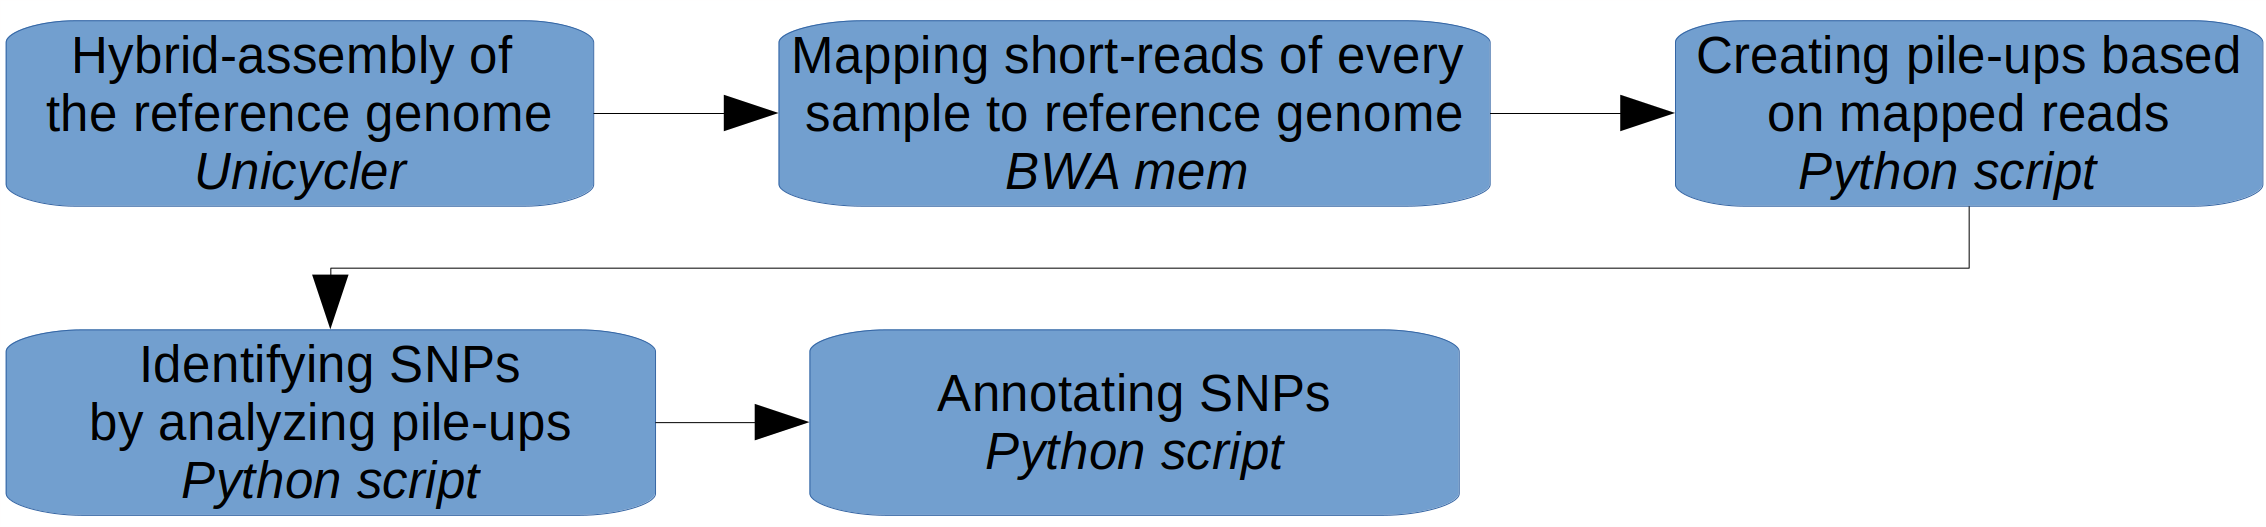
\includegraphics[width=0.9\textwidth]{pipeline.png}
	\caption{Bioinformatic pipeline used for the identification of mutations and affected genes/promoters.}
	\label{figure:pipeline}
\end{figure}
The foloowing pipeline was used to identify SNPs in isolate series which evolved resistance. This pipeline was based on Illumina and ONT sequencing data coming from multiple isolates which were taken while resistance evolved. In principle a hybrid-assembly of the genome was performed for the isolate with the lowest MIC. This genome was used as a reference in order to identify SNPs accumulated in the other isolates where resistance evolved. We also tried to provide annotation for the SNPs. 

\subsection{Creating a reference genome with annotation} 
As a first step we hybrid-assemblied the genome of the isolate with the lowest cefepime MIC of an isolate series with Unicycler \cite{wick_unicycler:_2017}. Every assembly was annotated with prokka which produced a genbank file for every reference genome \cite{seemann_prokka:_2014}. Additionally promoter regions were identified using the promoter prediction tool PePPER \cite{pepper}. PePPER is a tool which takes whole-genomes as an input and predicts promoter sequences. Those sequences were mapped against the reference genome using graphmap \cite{sovic_fast_2016}. Furthermore, a promoter data base hosted on EcoCyc was used. This database contains around 3800 experimentally validated promoters for \textit{E. coli}\cite{noauthor_smarttable_nodate}. The sequences from this database were downloaded and mapped against the reference genome with graphmap as well \cite{sovic_fast_2016}. 
\label{section:annotatiion_ref}.

\subsection{Mapping Illumina sequencing data of the isolate series to the reference genome}
As a second step of the pipeline the short-read Illumina sequencing data of every isolate was mapped against the reference genome of the isolate series. Mapping to the reference genome was done with BWE mem \cite{li_fast_2009}. This resulted in a bam file for every isolate of the series. Mapping all the Illumina reads provided us the information which base was present in every Illumina read mapped to a certain position to the reference genome. If the most abundant base of all Illumina reads at a certain position is different than in the reference genome a SNP was present. To make this information more accessible we calculated pile-ups as a third step of our analysis. 

\subsection{Calculating pile-ups}
Pile-ups are count matrices storing which base is present how many times at a certain position considering every mapped Illumina read. In order to produce those pile-ups we used a script called \href{https://github.com/nahanoo/ESBL\_project/pileup.py}{pileup.py}. This script extracted the base counts by going through every position of the sorted bam-file from an isolate. Pile-ups were calculated for every isolate of a series and all the pile-ups stored in a matrix stack.

\subsection{Identification of SNPs} 
We identified SNPs by comparing the most abundant base at every position of the matrix-stack with a script called \href{https://github.com/nahanoo/ESBL\_project/pileup.py}{analysis\_modular.py}. If the most abundant base varied between the isolate a SNP was identified. For the rest of the pipeline only SNPs were included where the coverage was at least 30 and the base frequency at least 0.8.

\subsection{Identifying genes and promoters affected by mutations}
As a last step of the pipeline we checked if annotation was available for the SNPs. For checking if a SNP affected a gene, we analyzed the genbank file with biopython \cite{cock_biopython:_2009}. To check whether a SNP affected a promoter region we analyzed the bam-files which were created with the promoter sequences from PePPER and EcoCyc. We checked if a SNP was located between a start or end position of a mapped promoter sequence. 

\section{Assembling the morbidostat}
We experimentally evolved resistance to cefepime with ESBL \textit{E. coli} strains using a morbidostat. We assembled an adapted version of Topraks built differing mainly in its pump system, controlling unit and software\cite{toprak_building_2013}. Hardware which was not commercially available was built by the in-house mechanic and electronic workshop.

\begin{figure}
	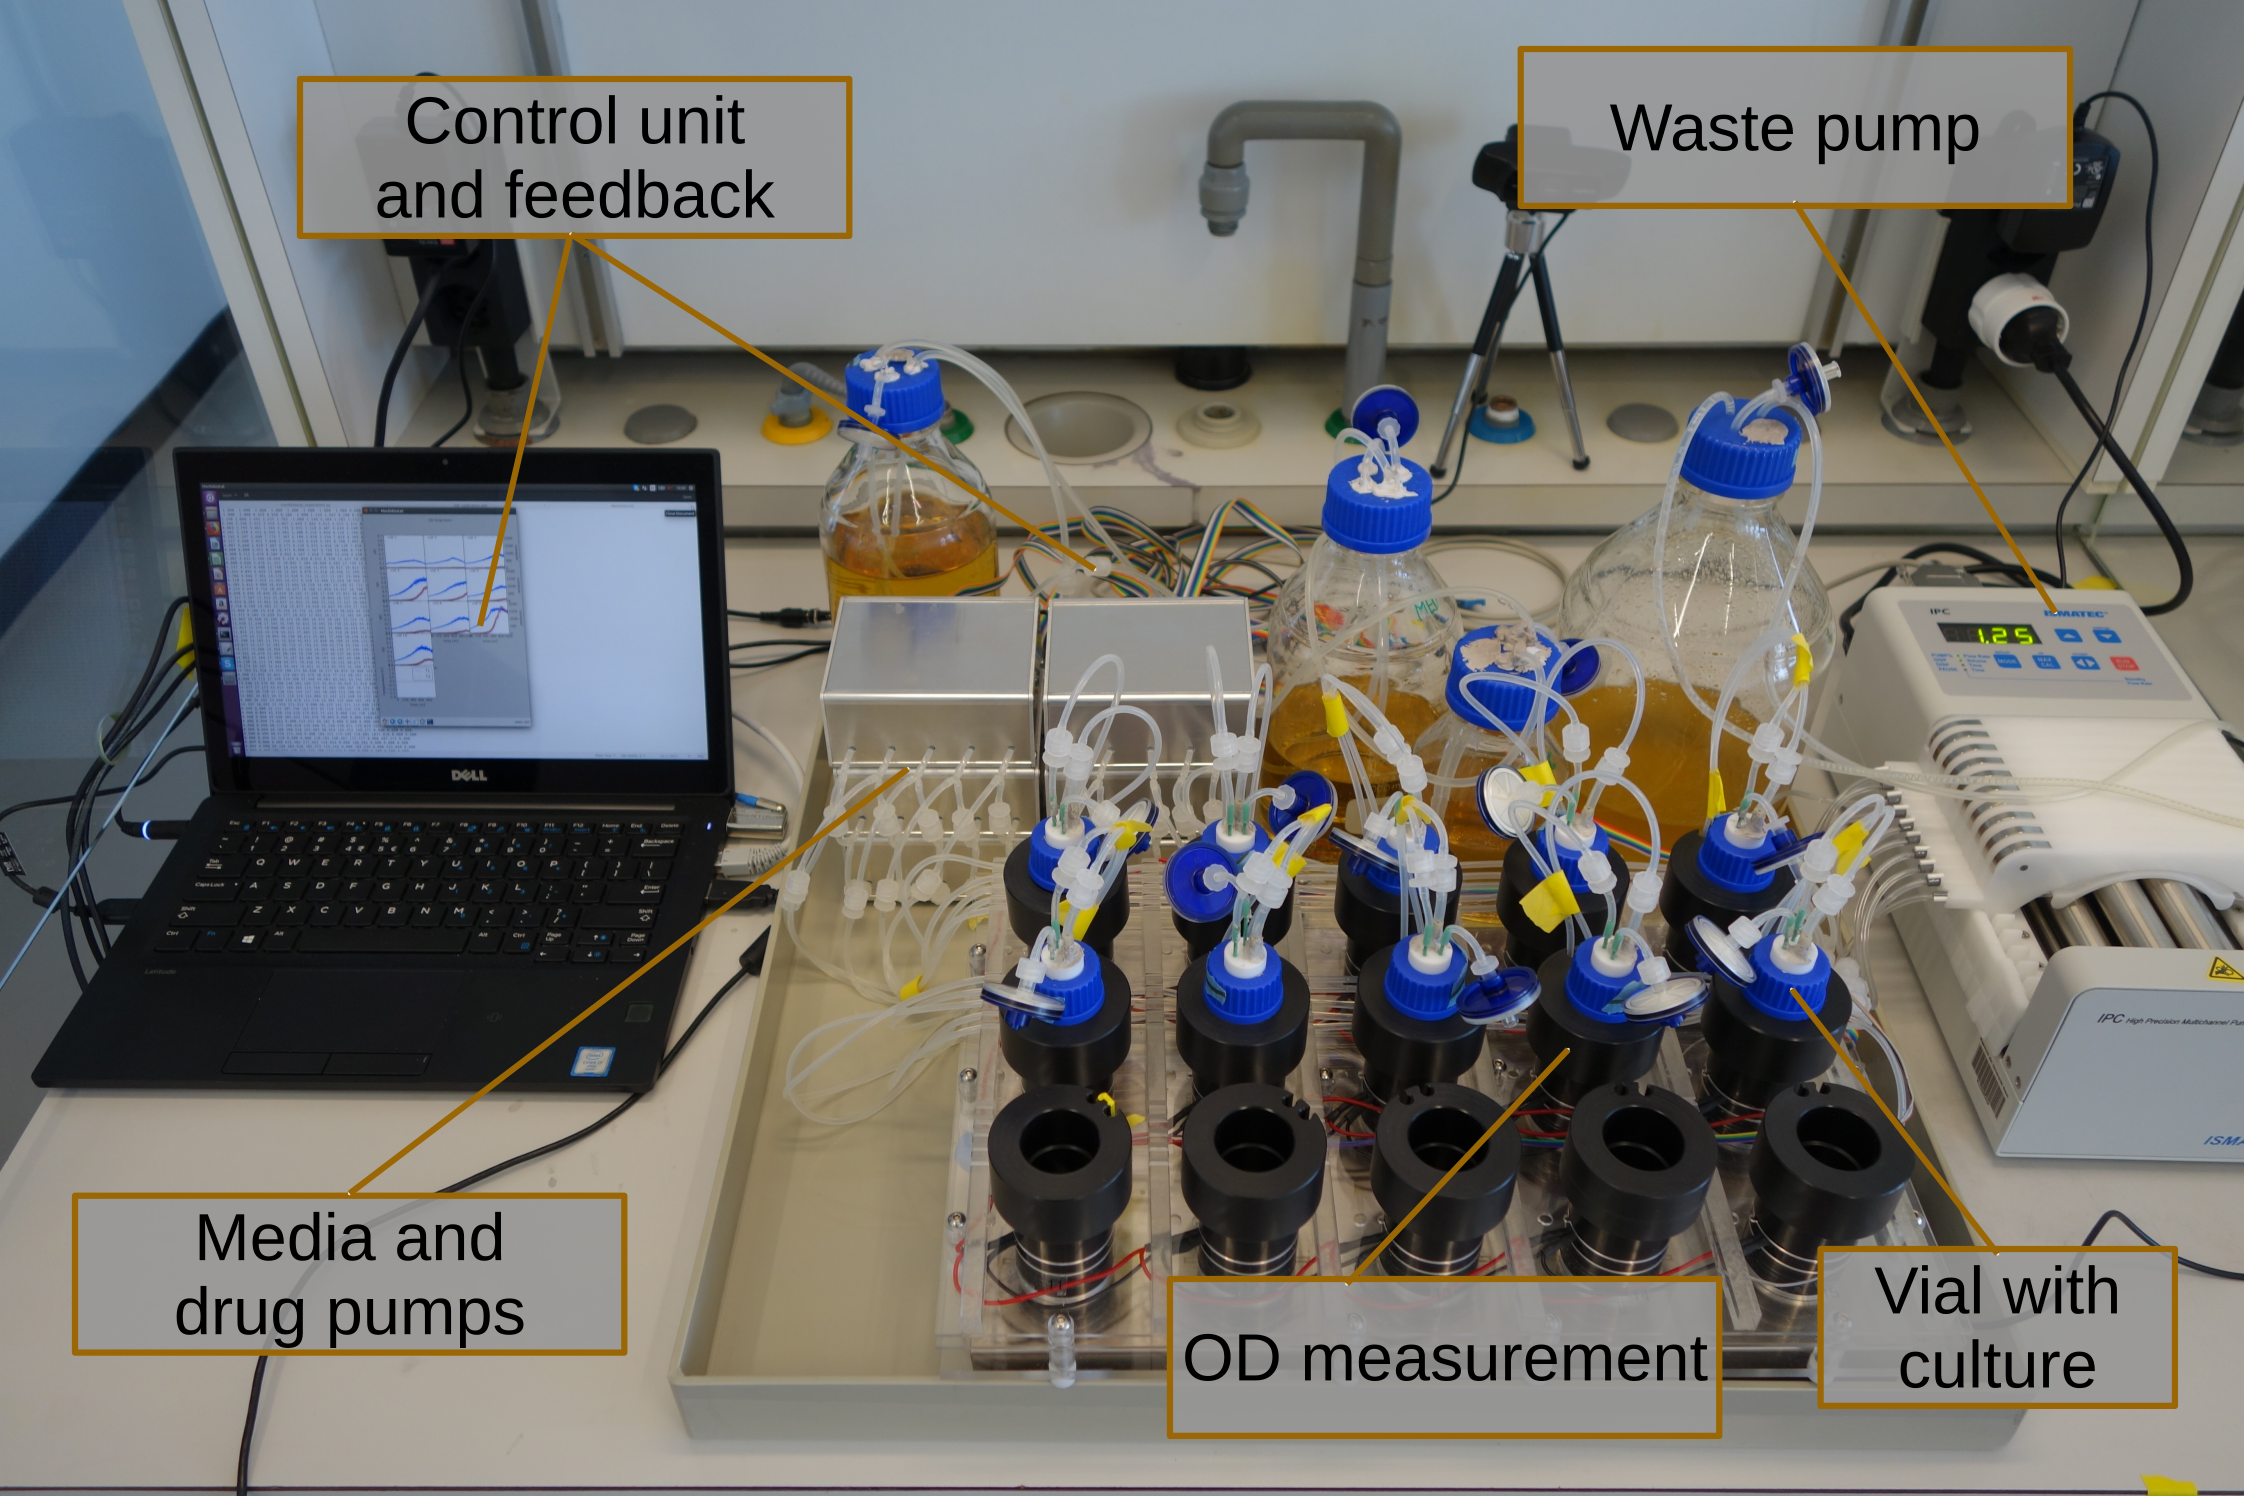
\includegraphics[width=0.7\textwidth]{setup_annotated_inksacpe.png}
	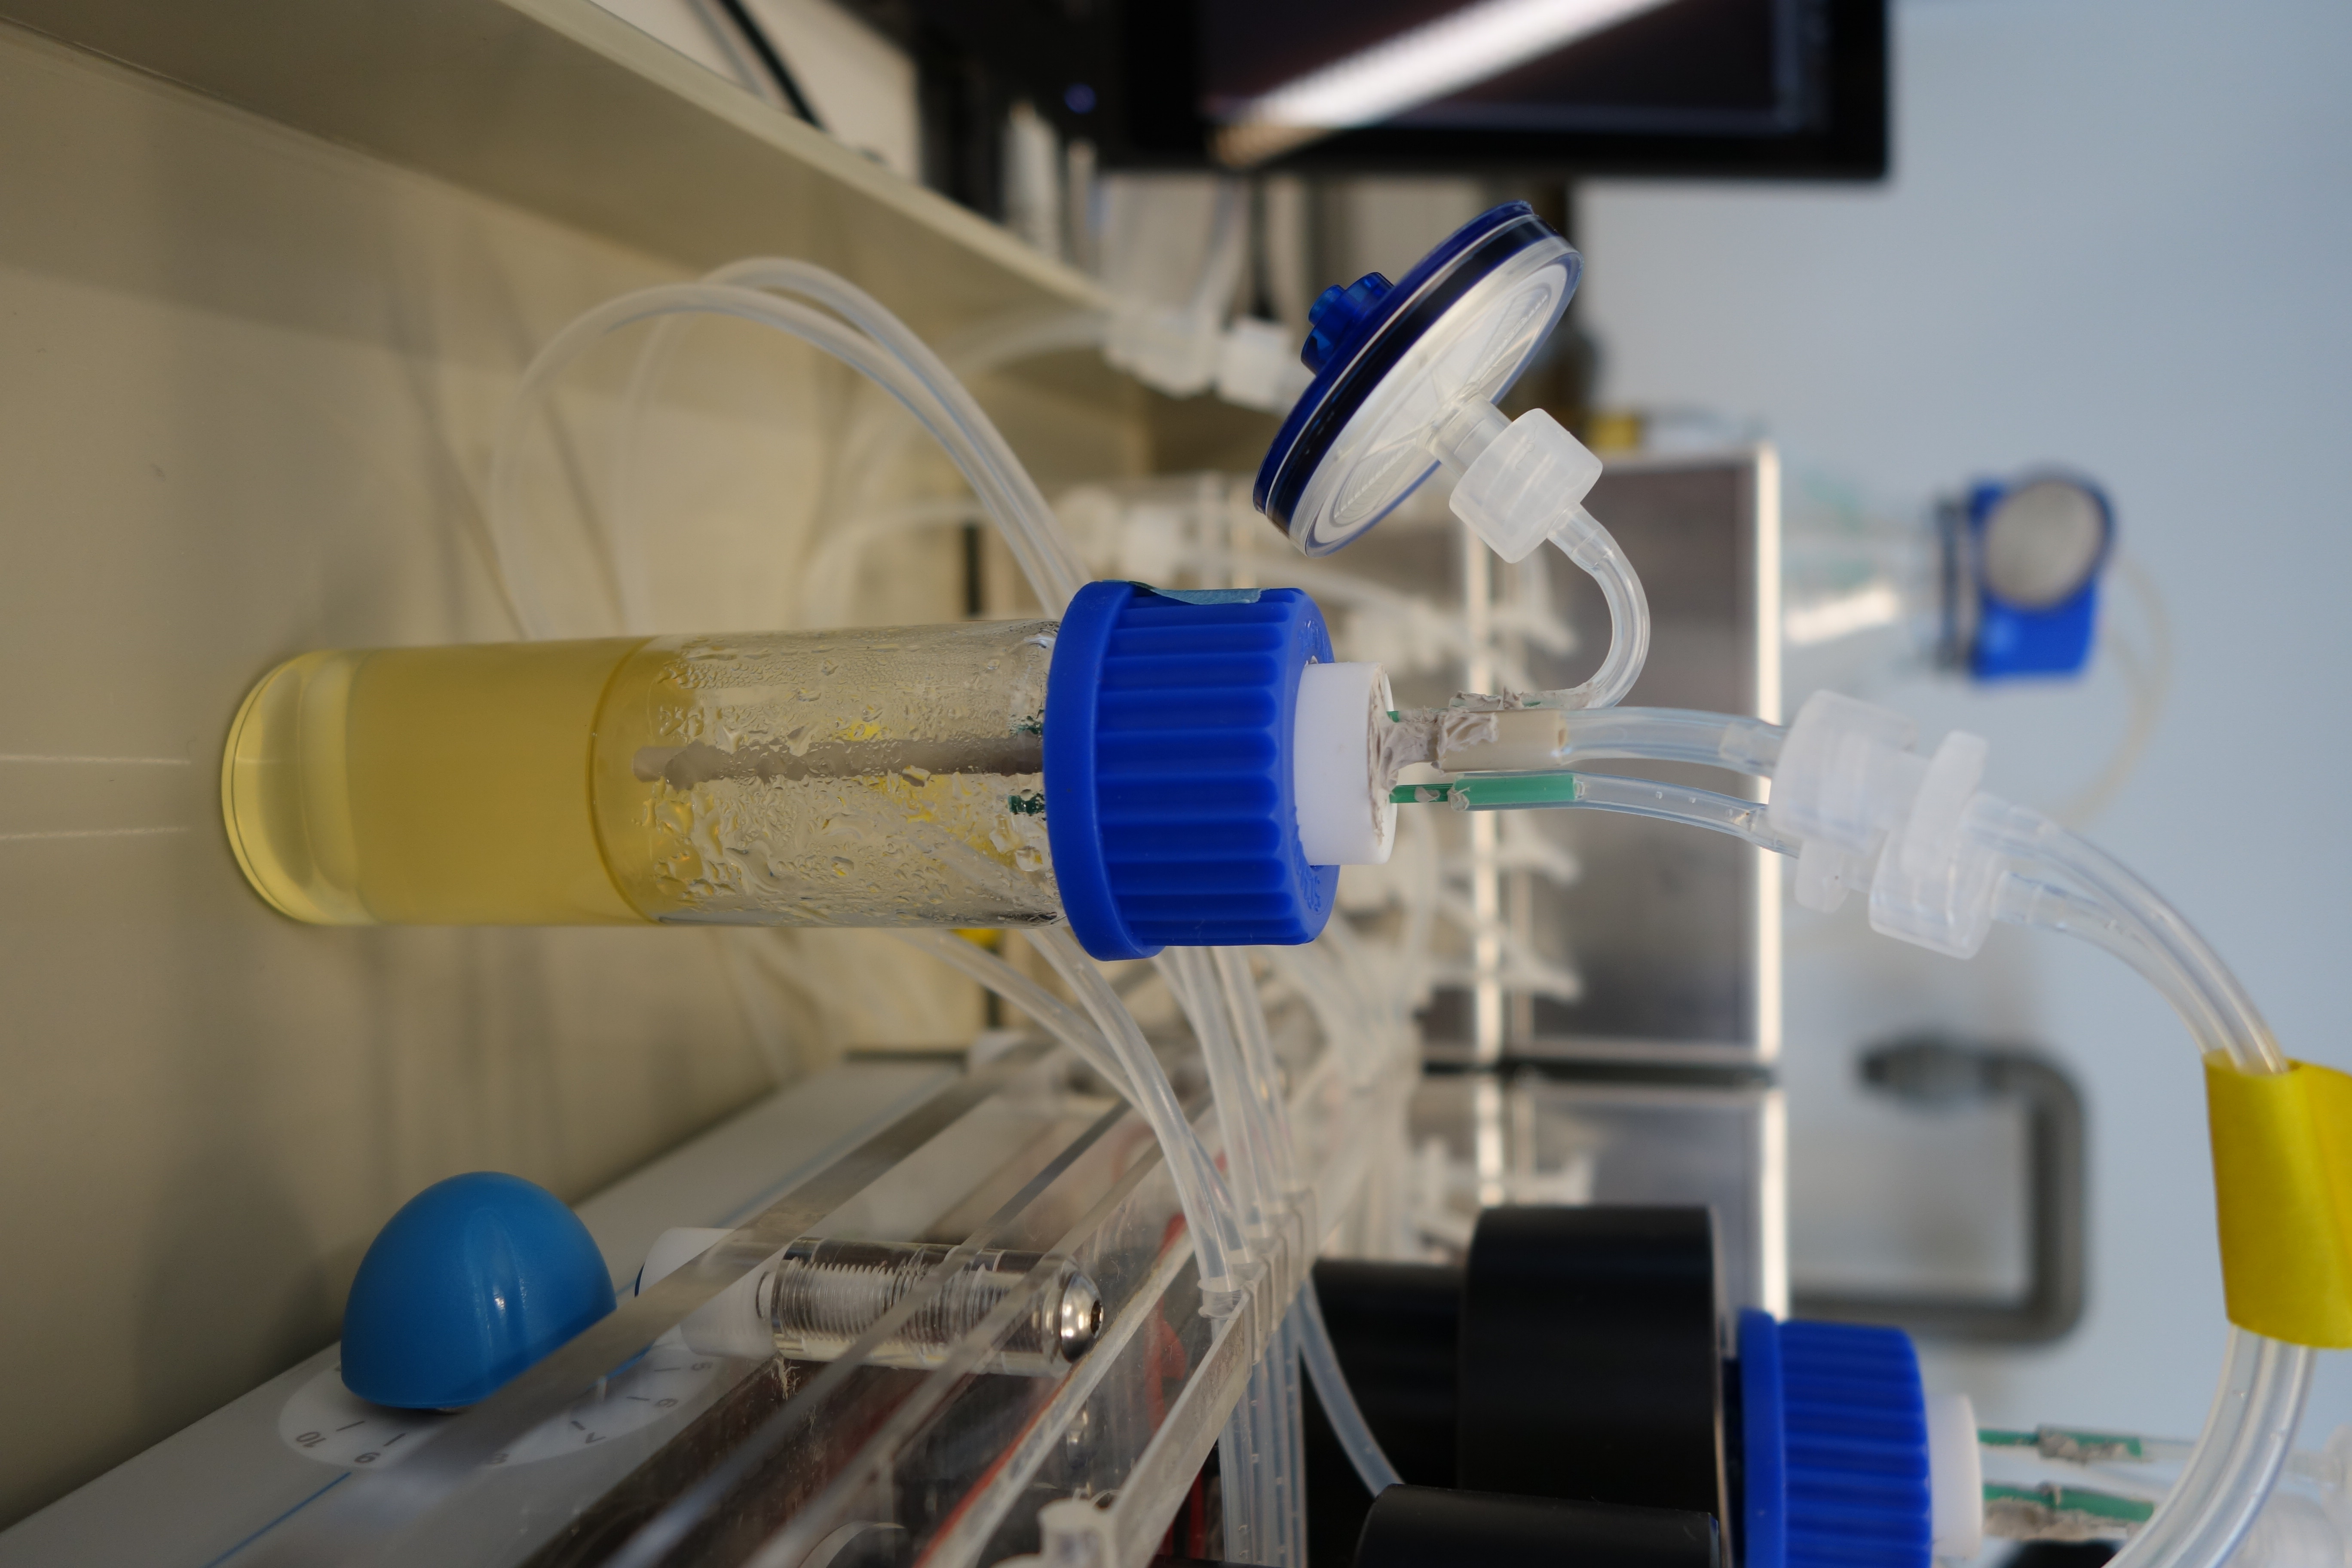
\includegraphics[width=0.4\textwidth,angle=90]{vial.JPG}
	\caption{Left: Overview of the morbidostat setup. Vials were placed on magnetic stirrer and connected to three drug injecting pumps and one waste removal pump. A microcontroller was connected in serial to a PC, which allows to computer control drug injections and OD measurements. Right: One vial with all the inlets.}
	\label{figure:morbidostat_setup}
\end{figure}  
Figure \ref{figure:morbidostat_setup} shows the morbidostat setup.
As a base for our build we used a magnetic stirrer with 15 slots. On that stirrer we placed three layers of acrylic glass through which we inserted black plastic rings which acted as our vial holders and optical density (OD) measuring units. 
The vials placed in the vial holders had three inlets as shown in Figure \ref{figure:morbidostat_setup}. One inlet was used to inject media or antibiotics, one for removing volume exceeding the culture volume and the last one to mount an air filter for pressure equilibration. \\
To test the hardware, we built the morbidostat in the open as shown in Figure \ref{figure:morbidostat_setup}. For the actual experiments we placed the morbidostat inside a hypoxi-station in a bio safety lab 2. This allowed us to culture the bacteria at 37 \degree C but also to increase the safety. 


\subsection{OD measuring units}
For measuring the ODs we sent a ray of light through the cultures. This ray was scattered by the cells meaning that the ray was thrown off by the cells in multiple directions. With the help of a phototransistor we could measure the scattering with analog pins of the microcontroller. Because the scattering was proportional to the cell density, we could translate the scattering into an OD by calibration. \\
One OD measuring unit integrated in the vial holder is shown in Figure \ref{figure:OD_unit}. Every unit consisted of a vertical-cavity surface-emitting laser (VCSEL) and a phototransistor. We chose OPB608V as a VCSEL with a peak wavelength of 890 nm and PT 333-3C as a phototransistor, both from TT electronics. For each unit the VCSEL and the phototransistor were placed in a 135 \degree \space angle inside the vial holder. Both components were in direct contact with the glass vial.
The 15 OD measuring units were divided into three groups of five units which corresponds to one row of vials of the morbidostat. For every group the VCSELs and phototransistors were both connected to independent 5 V circuits. The circuits of one group are illustrated in the left Figure \ref{figure:OD_cirguit}, where the VCSEL circuit is shown orange and the phototransistor circuit in blue. \\
The VCSELs were constantly on sending rays of light through the cultures. When an OD measurement was initialized the scattering was detected with the phototransistors. Light reaching the phototransistor caused an opening in the semiconductor from the phototransistor which led to an amplification of the current. This current reached a potentiometer connected in serial over which we measured the voltage with an analog pin of the microcontroller. The opening of the semiconductor altering the measured voltage correlated with how much light reached it. More cells caused more scattering and more light reaching the semiconductor. Therefore, there was a linear correlation between the measured voltage and the cell density in the suspension. \\

\label{section:OD}
\begin{figure}
	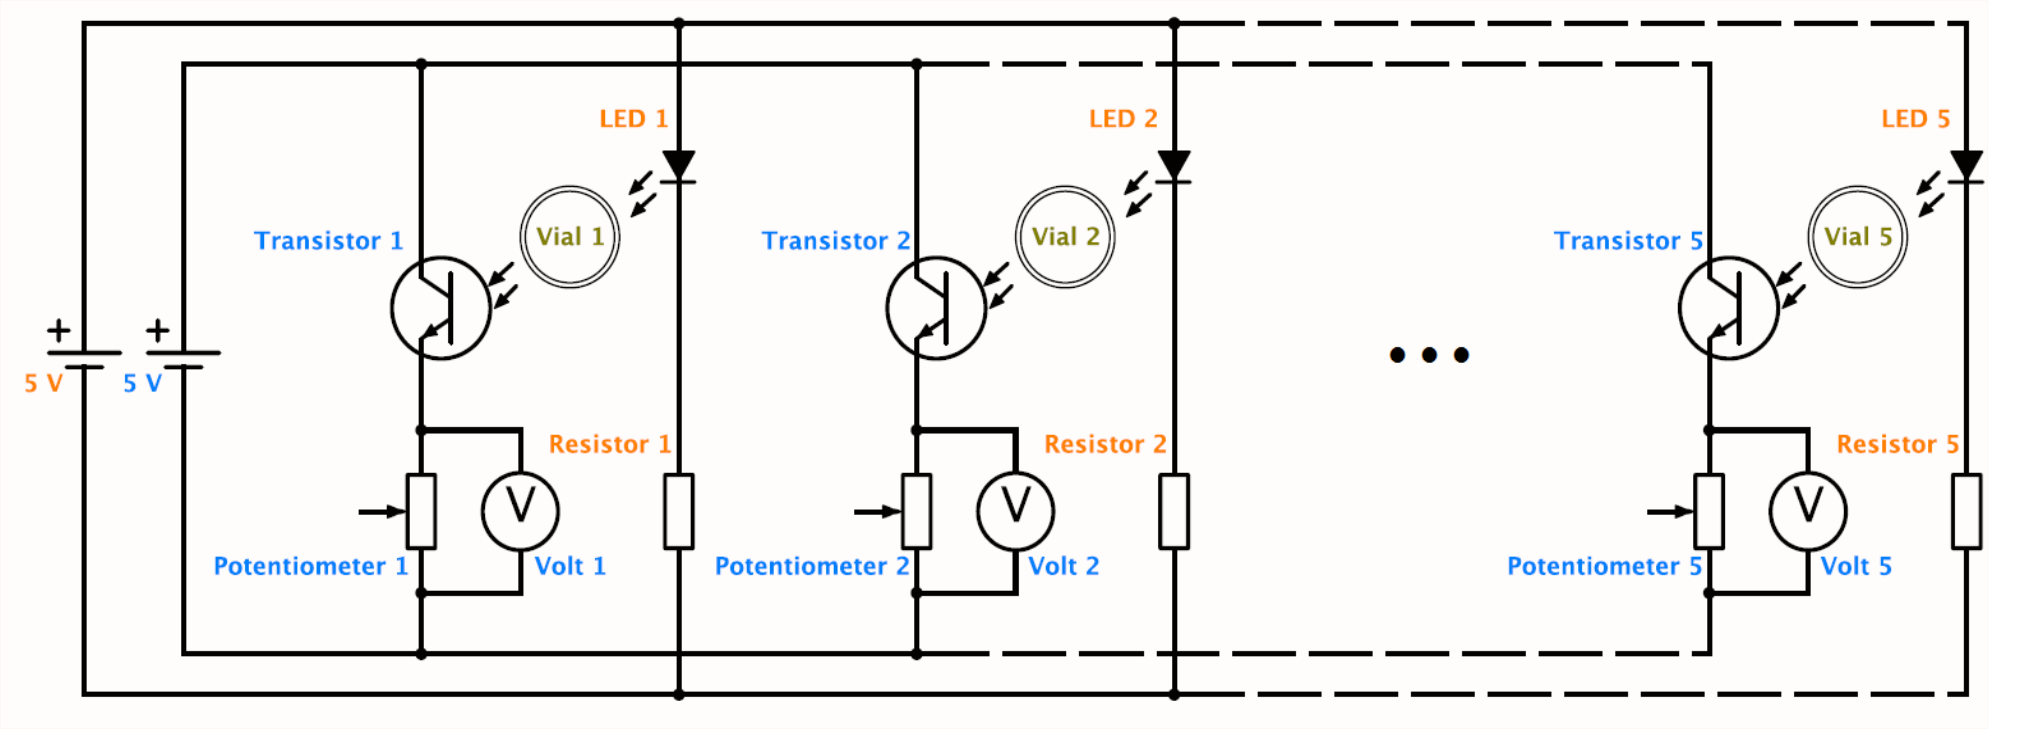
\includegraphics[width=0.6\textwidth]{OD_setup.png}
	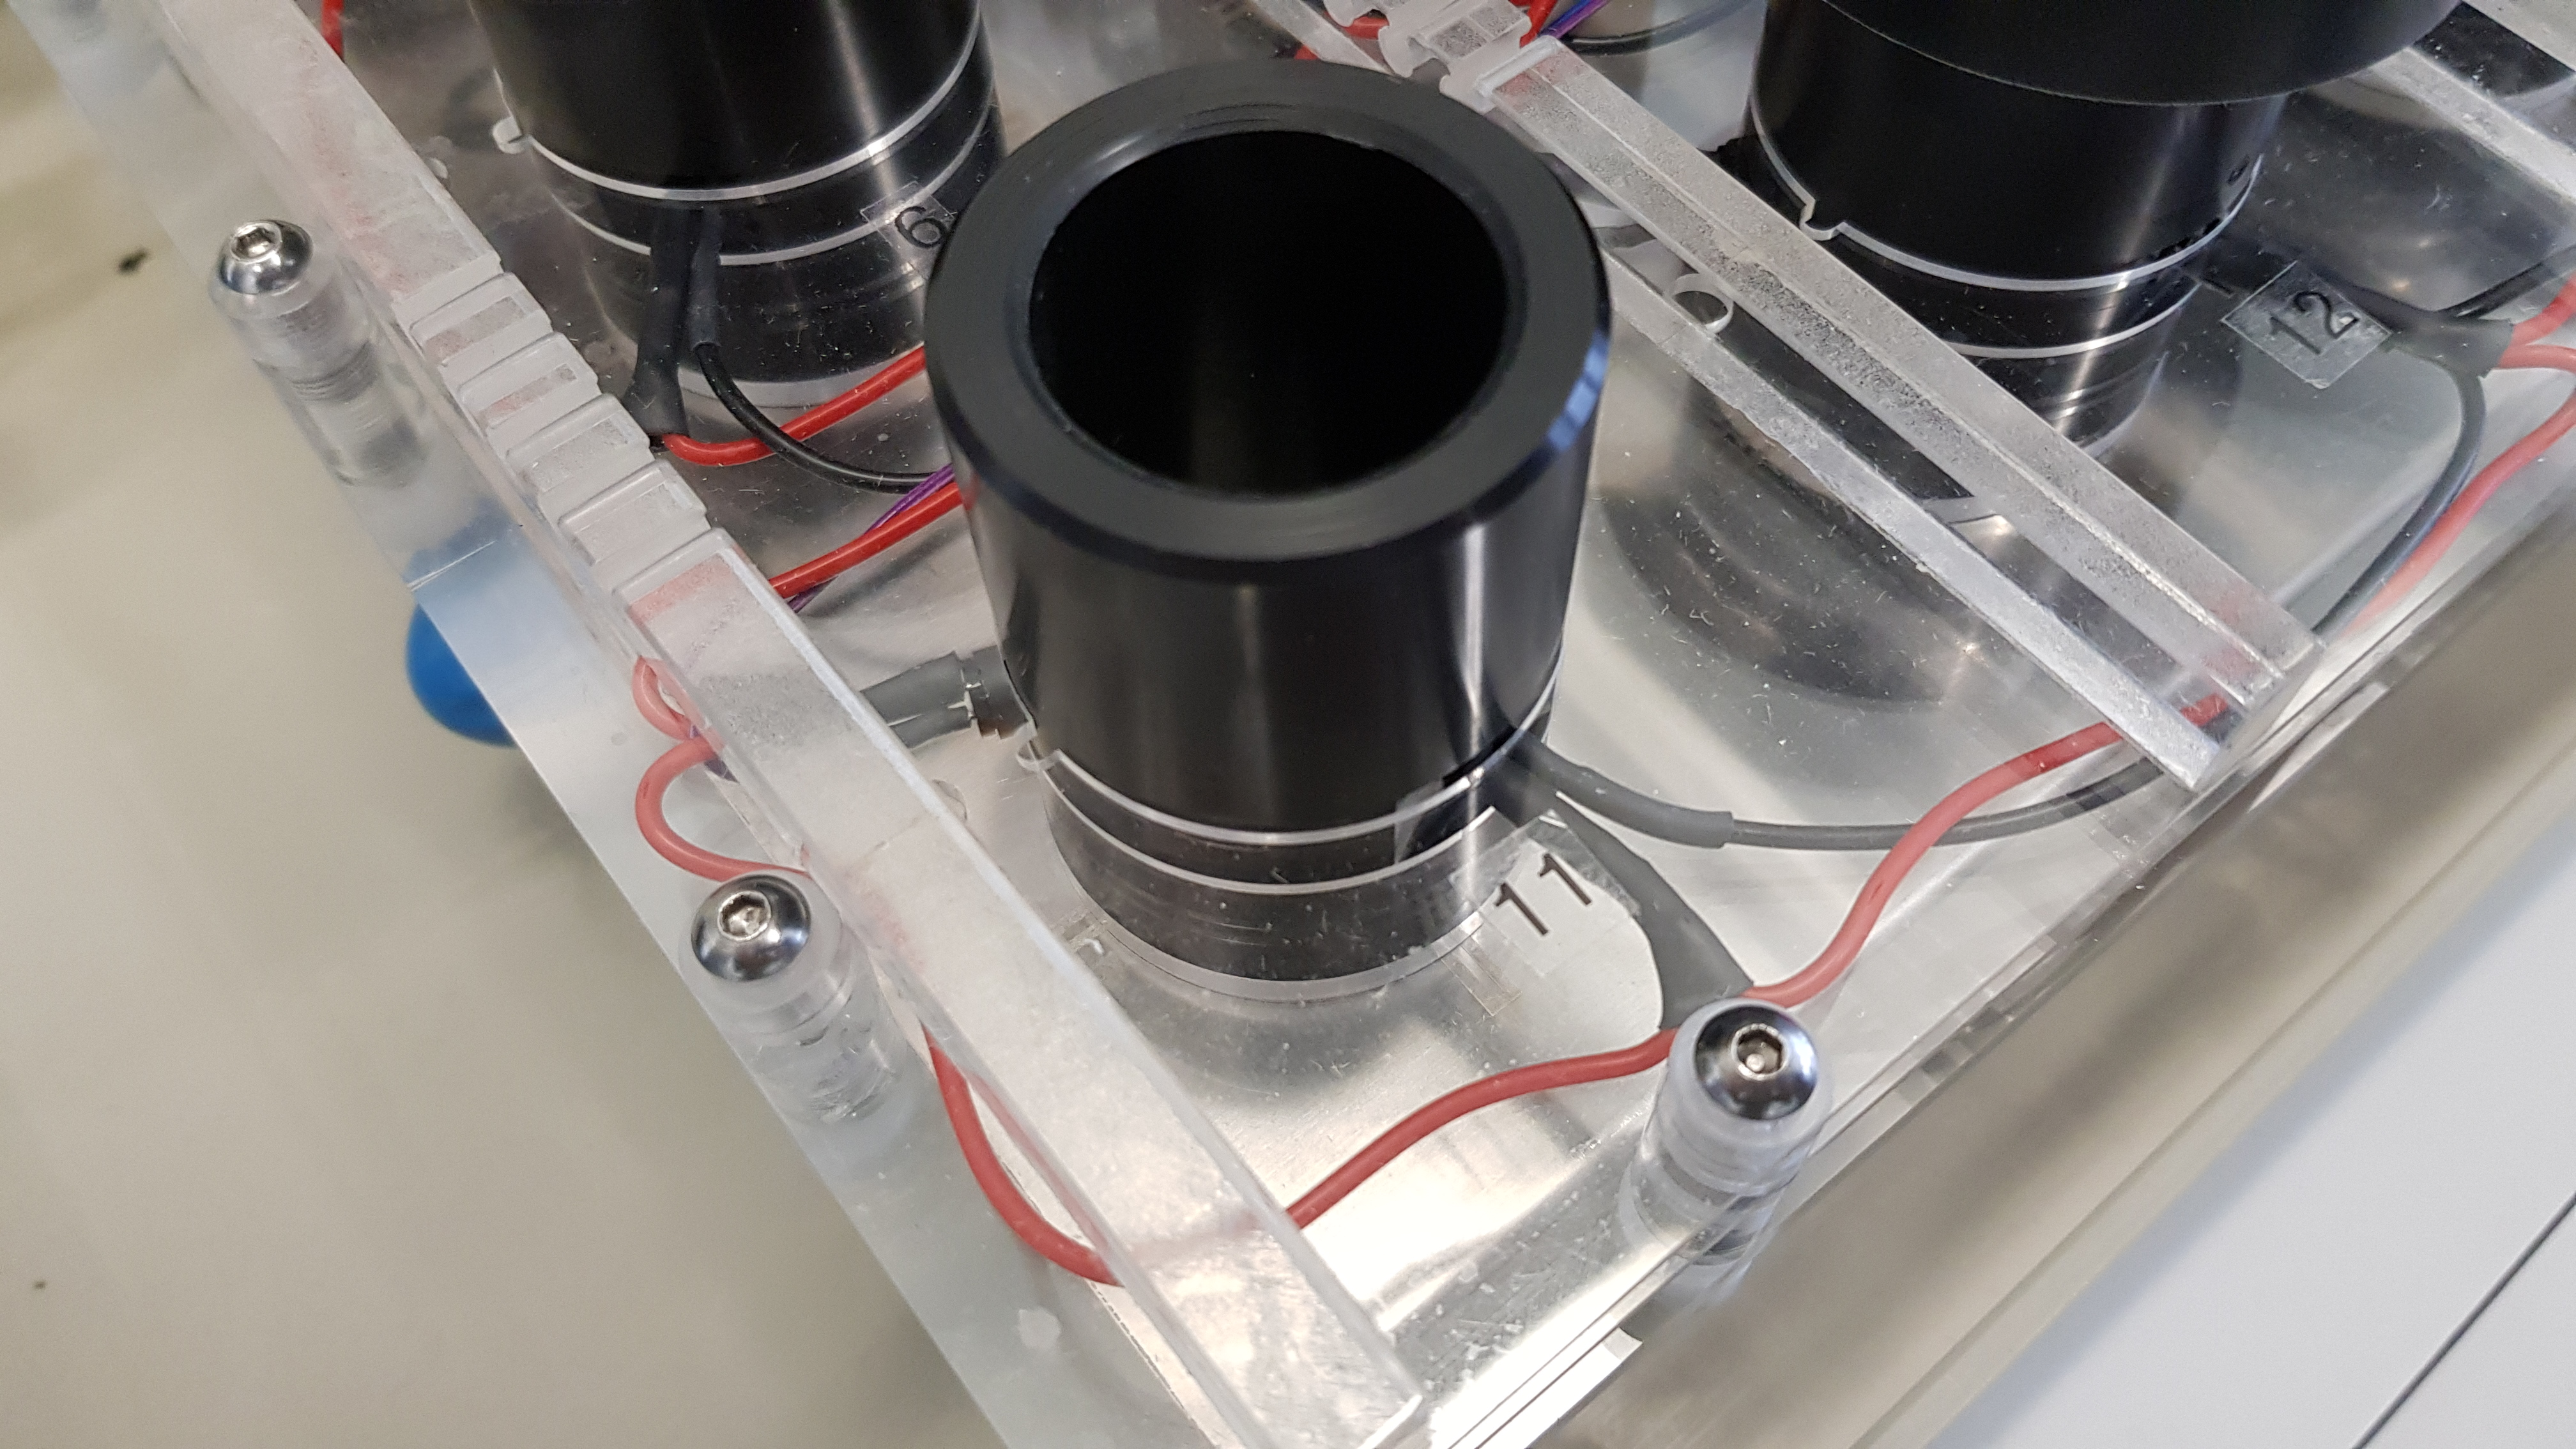
\includegraphics[width=0.3\textwidth]{OD_unit.png}
	\caption{Left: Circuit for parallel connected VCSELs (orange). Each VCSEL is connected in serial with a 220 \textOmega \space resistor. The circuit of the phototransistors is shown in blue. The phototransistors are connected in parallel. Each phototransistor is connected to a potentiometer in serial over which the voltage is measured with an analog pin of the microcontroller.}
	\label{figure:OD_cirguit}
	\label{figure:OD_unit}
\end{figure}

\subsection{Pumps and tubing} 
\begin{figure}
	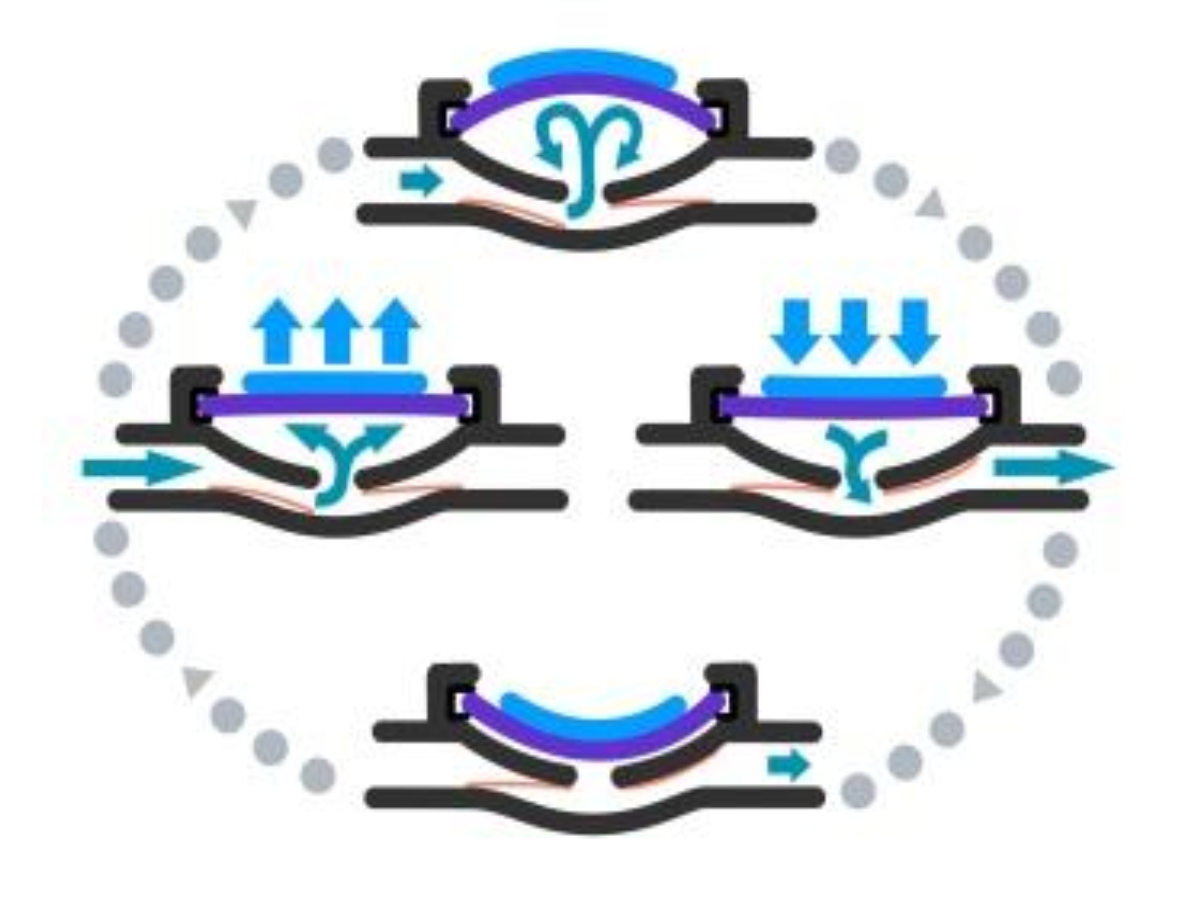
\includegraphics[width=0.2\textwidth]{piezo.png}
	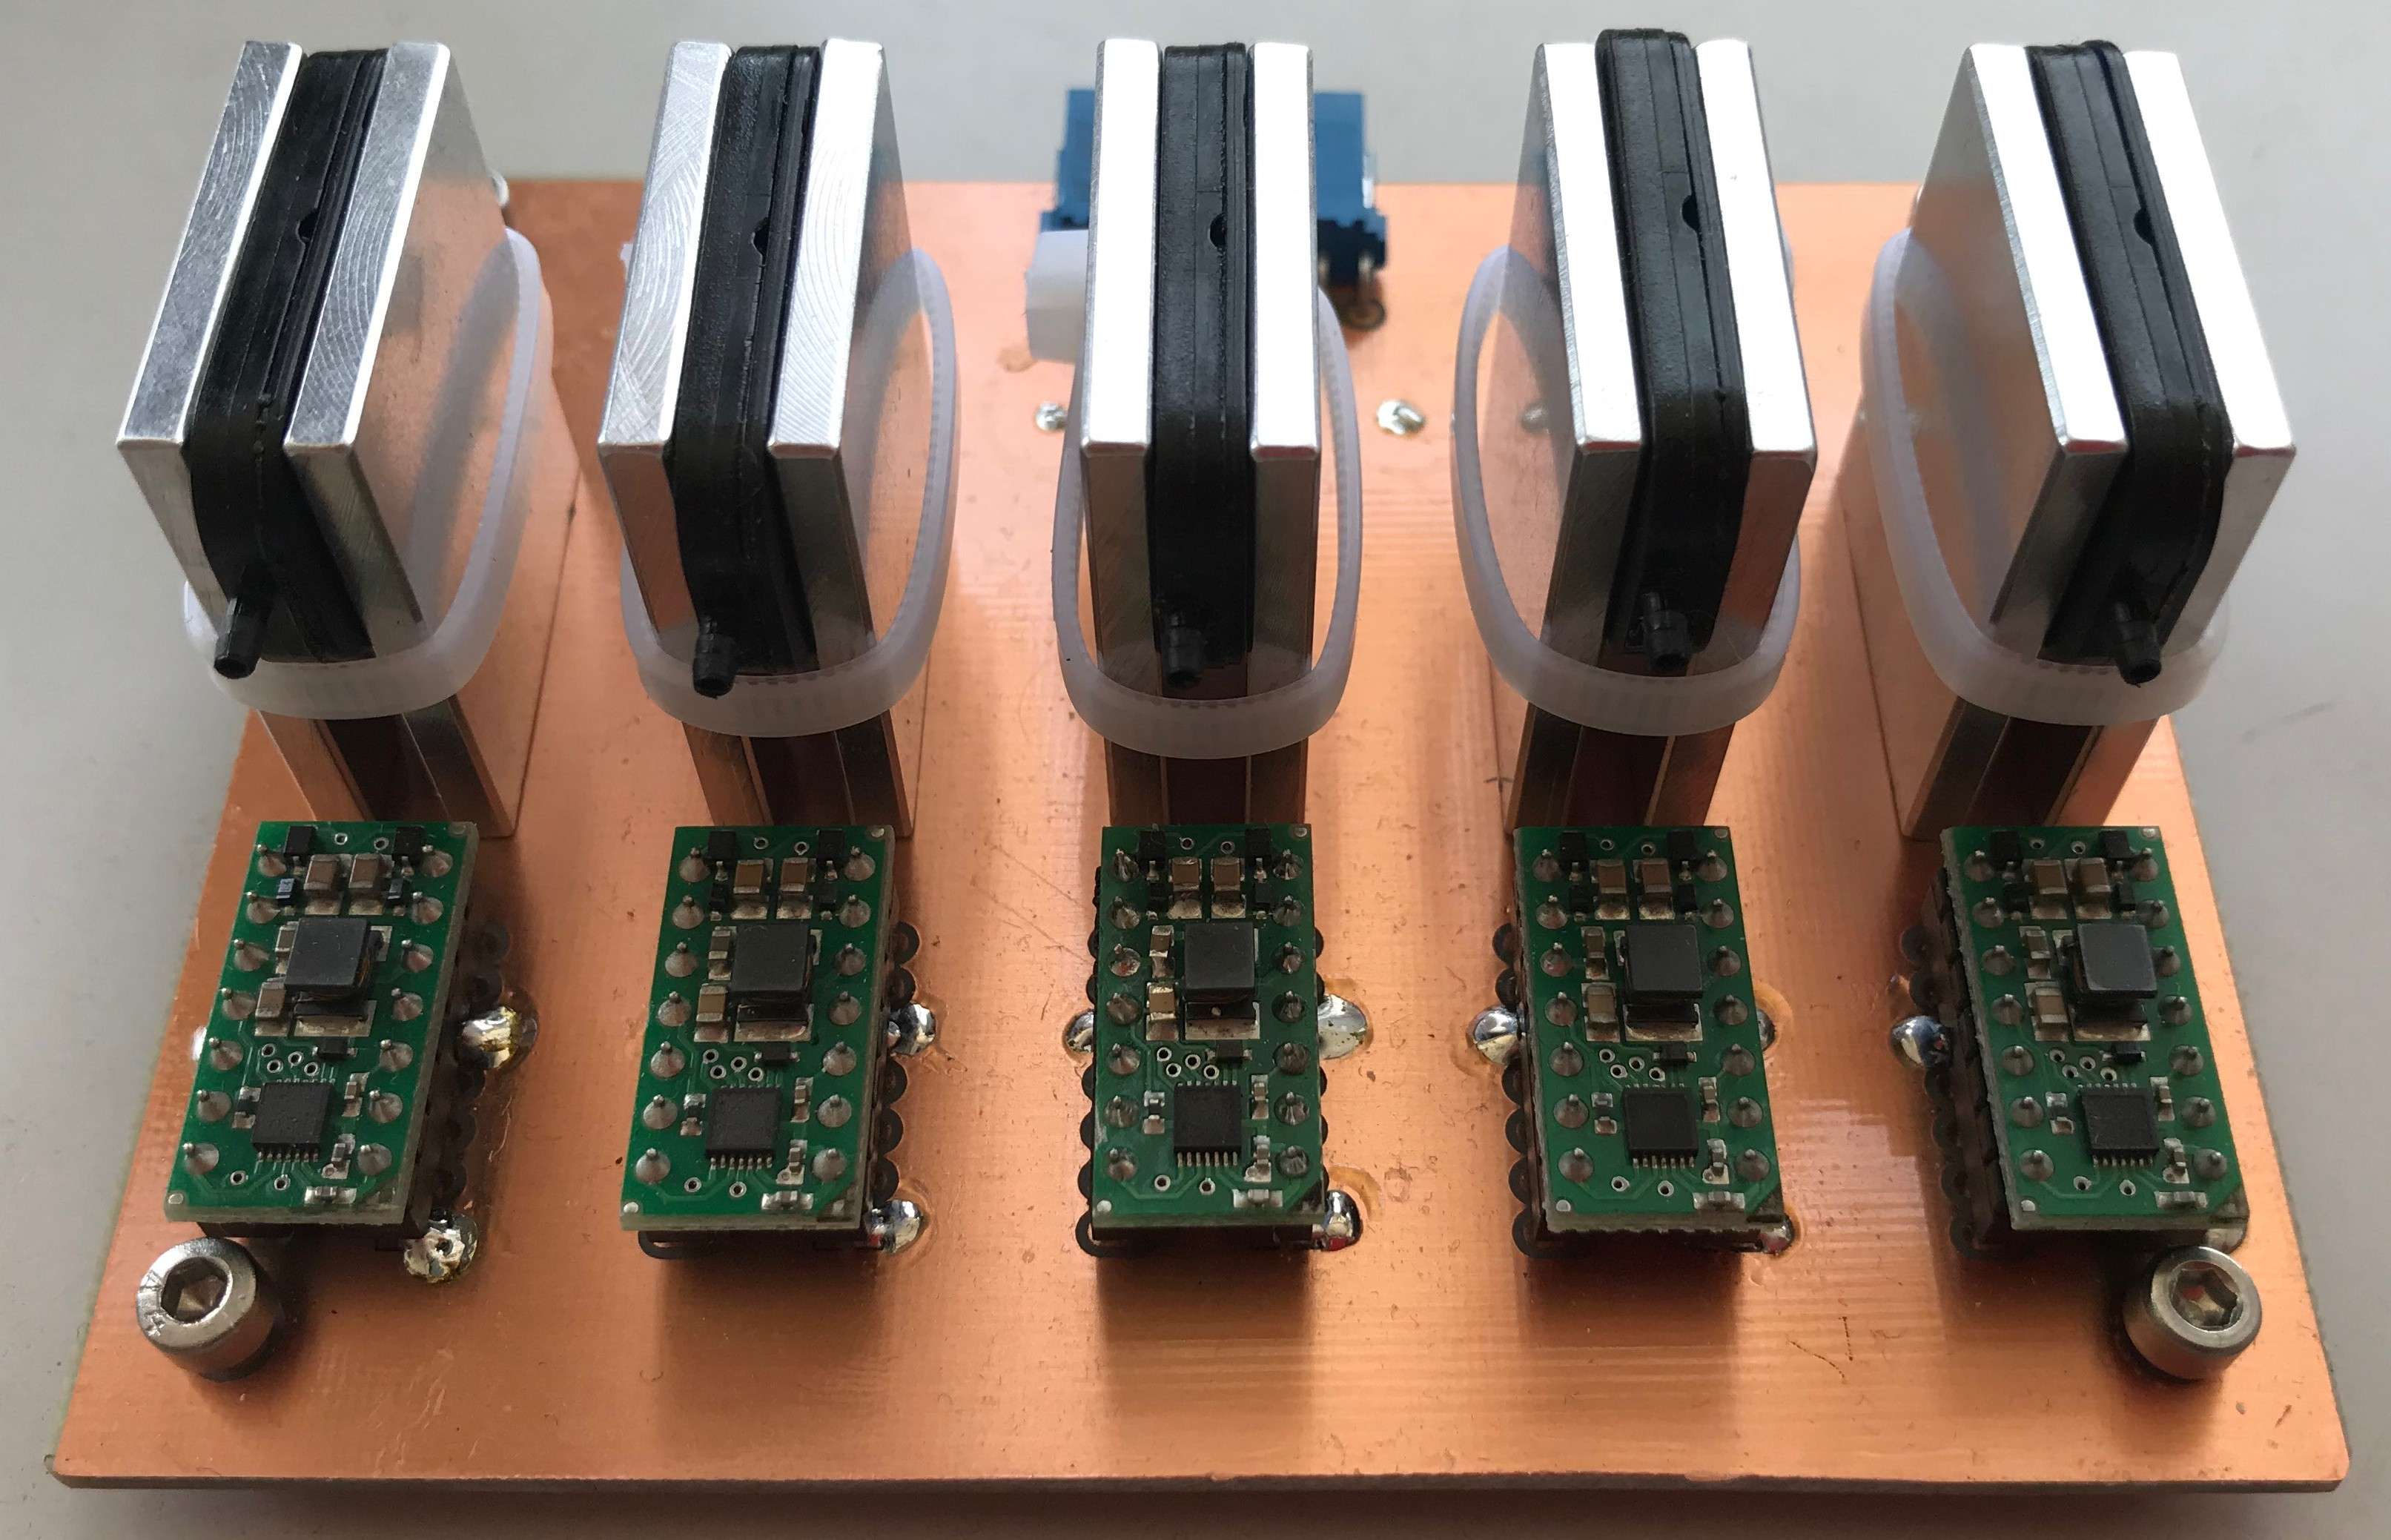
\includegraphics[width=0.4\textwidth]{board.JPG}
	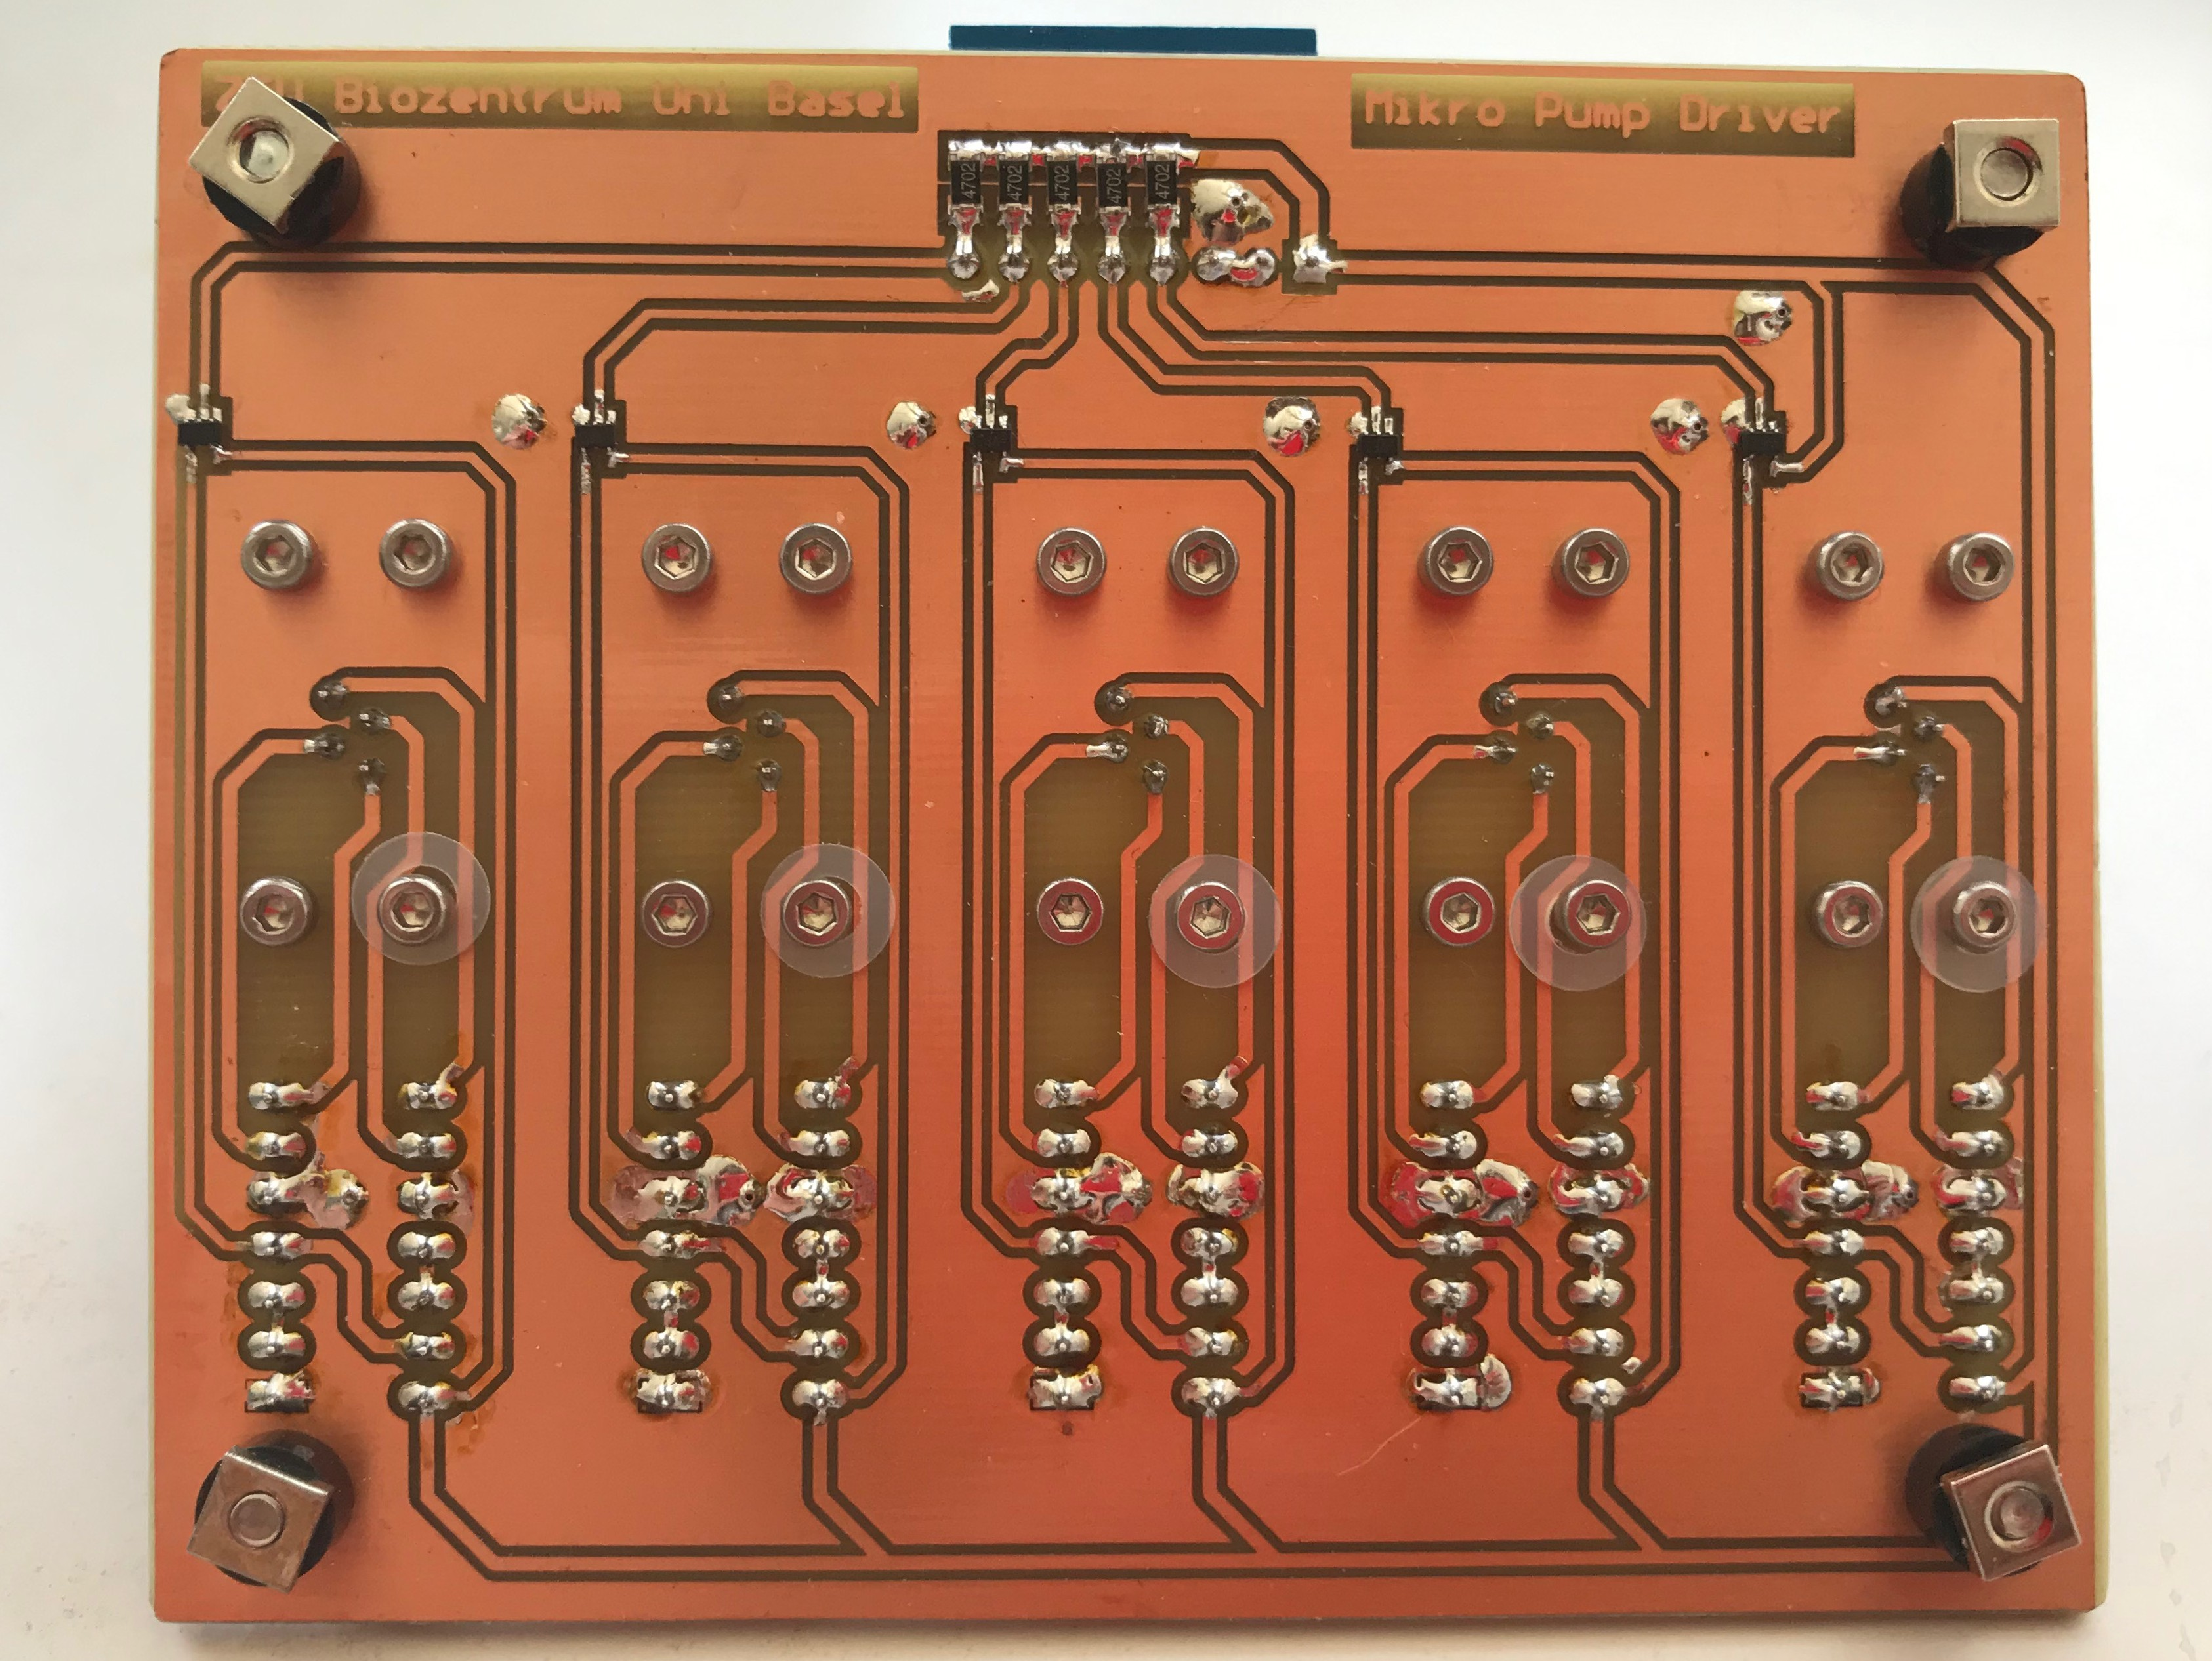
\includegraphics[width=0.4\textwidth]{board_below.png}
	\caption{Left: Principle of the piezo pumps. Top state: Piezo ceramic (purple) mounted on a membrane (blue) is relaxed. Left valve is open (orange), right valve  is closed, liquid enters. Right and bottom state: Voltage is applied to the piezo ceramic deforming the membrane resulting in a down stroke. Left valve is closed, right valve is open Liquid exits to the right. Voltage decreases again and the piezo ceramic enters its relaxed state again \cite{piezo_pumps}}. Middle: Top view of a circuit board with five pumps and five controllers. Right: Bottom view of a circuit board. 
	\label{figure:pumps}
\end{figure}
\begin{figure}
	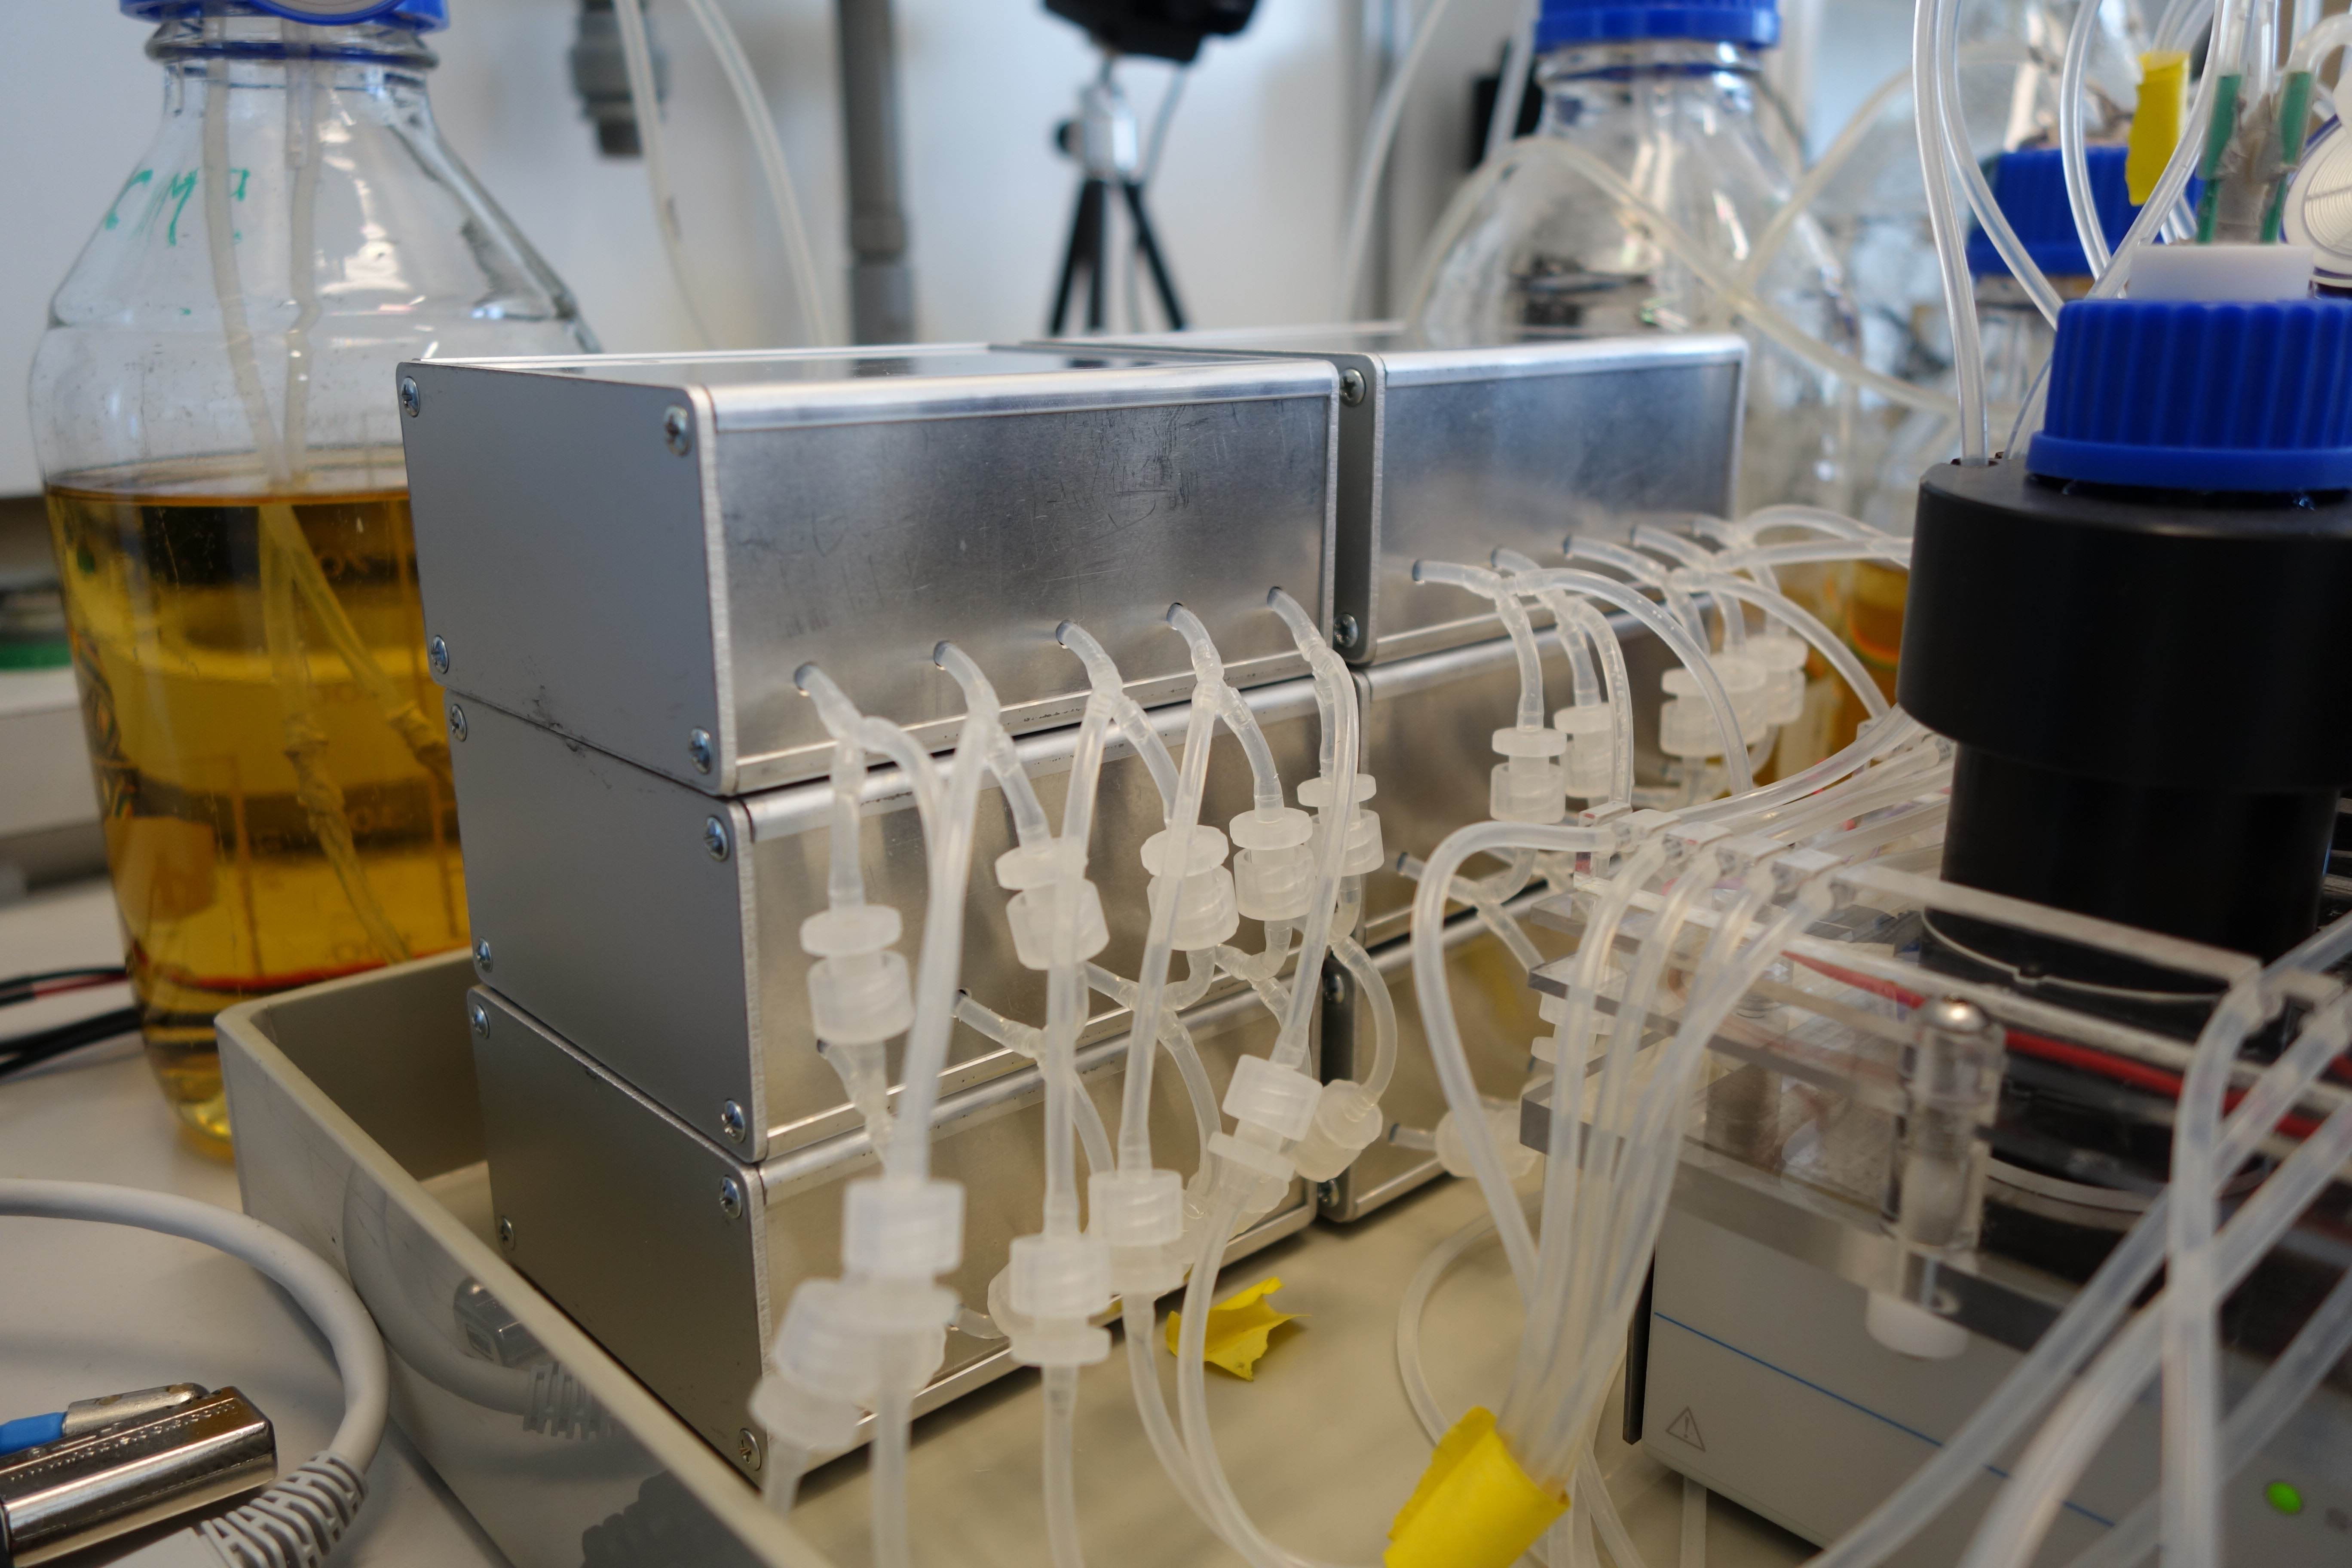
\includegraphics[width=0.5\textwidth]{pump_blocks.JPG}
	\caption{Three pump boxes with five pumps and controllers stacked on top of each other. The outlets of the pumps were connected column by column and led to the vials.}
	\label{figure:tubing_setup}
\end{figure}
Every vial was connected to three injecting pumps. One pump was responsible for injecting media, one for injecting a low-concentrated antibiotic and one for injecting a high-concentrated antibiotic. Mixing of desired antibiotic concentrations was possible by controlling the run times of the pumps.
We chose mp6 pumps from microComponents because of their very compact build. The functional principle of the pumps is shown in the left Figure \ref{figure:pumps}. We achieved a steady flow rate of the pumps with the mp6-OEM controller from microComponents. On one circuit board five pumps with five mp6-OEM controllers were mounted which is shown in Figure \ref{figure:pumps}. Each mp6-OEM controller was connected to one pump, a 5 V power supply, a ground and a digital pin of the microcontroller which allowed computer controlling the run times of every pump. The circuit boards were mounted in a metal box and three of those boxes stacked on top of each other which is shown in Figure \ref{figure:tubing_setup}. By packing five pumps in a box and stacking three boxes on top of each other we were able to connect one row of vials to the whole range of antibiotic concentrations with one stack. Pumps of the lowest box were connected to media, pumps of the middle box to a low-concentrated antibiotic and the pumps of the top box to a high-concentrated antibiotic. We connected the outgoing tubes of the pumps from one stack column by column resulting in one outgoing tube per column as shown in Figure \ref{figure:tubing_setup}. Those tubes were led to the vials. This way we connected one vial with three pumps providing all concentrations of antibiotic and media with just one tube leading to the vial.\\
Every vial was also connected to a 16-channel peristaltic pump which removed volume exceeding the culture volume through the gray tube shown in the right Figure \ref{figure:morbidostat_setup}. 

\subsubsection{Computer controlling the pumps}
In order to control the run times of the pumps a pin of every mp6-OEM controller was connected with a digital pin of the microcontroller. If the pin of the mp6-OEM controller received a voltage of 5 V the pumps were off, if the pin was set to ground the pumps were on. \\
When we set the digital pins of the microcontroller to ground there was still a low current flowing, resulting in a small voltage. The mp6-OEM controllers reacted very sensitive to this small voltage leading to weird behavior of the pumps. We solved this by inserting a pull-down resistor between the digital pins of the microcontroller and the ground which is shown in Figure \ref{figure:pumps}. Additionally an inverter was connected in serial to the digital pins. To turn on a pump the digital pins of the microcontroller was set to 5 V. The inverter connected in serial set the signal at the pin of the mp6-OEM to ground and the pumps. Run time control was possible by setting the digital pins to 5 V for the desired time.
The 16-channel peristaltic pump was also computer controllable because the pump was also connected to a digital pin of the microcontroller.
\label{section:pumps}

\subsection{Controlling the morbidostat}
As a microcontroller we used an Arduino mega 2560 flashed with an arduino-script called \href{https://github.com/nahanoo/ESBL\_project/}{arduino\_morbidostat.ino}, which allowed us to change the state of digital pins or measuring voltages of analog pins. The microcontroller itself was controlled by a laptop where two python scripts were running. The python script \href{https://github.com/nahanoo/ESBL\_project/}{morbidostat\_experiment.py} decided which analog pins were measured and which digital pins were set to high for how long. Those tasks were grouped in cycles and repetitively executed. Additionally this script was responsible for storing ODs and injected antibiotic concentrations. We used a second python script called \href{https://github.com/nahanoo/ESBL\_project/}{arduino\_interface.py} to enable the communication between the laptop and the microcontroller. Commands for the microcontroller initialized by \href{https://github.com/nahanoo/ESBL\_project/}{morbidostat\_experiment.py} were encoded in a string by \href{https://github.com/nahanoo/ESBL\_project/}{arduino\_interface.py} which was transmitted to the microcontroller via a serial USB connection. The microcontroller interpreted the string and executed the encoded commands. \\
We implemented three modes for the morbidostat in \href{https://github.com/nahanoo/ESBL\_project/}{morbidostat\_experiment.py}. Those being the continuous mode which we used for continuous inhibition of the cultures, a growth rate mode where growth rates with no injections were recorded and a fixed OD mode where the OD of a culture was fixed to a certain OD by dilution with media. \\   

\subsubsection{Tasks of a continuous morbidostat cycle}
As for every mode the continuous mode consisted of several tasks grouped in one cycle. Shown in Figure \ref{figure:flowchart} as a first step the microcontroller measured the voltages of the analog pins connected to OD measuring units for a defined cycle time (typically being 10 minutes). Those voltages were constantly sent to the laptop where they were translated to ODs which were saved. After the cycle time the program fit a line to the OD measurements of a cycle for every vial. Using this fit the growth of every vial was calculated and stored. Additionally the measured ODs of a cycle where averaged and stored as well. Then a feedback algorithm calculated how much drug to inject into which vial. Shown in Figure \ref{figure:flowchart} the last step of a cycle was to translate the calculated antibiotic concentration into run times of the three pumps connected to a vial. The run times were sent to the microcontroller. The microcontroller turned on the pumps for the calculated time and after removing volume exceeding the culture volume with the peristaltic pump one cycle was finished. The injected volume was the same for every morbidostat experiment, which was controlled with the dilution factor.  \\
The commandflow of the growth rate mode was very similar just that the feedback function was not executed and therefore no fluids were injected into the vials. For the fixed OD mode another function instead of the feedback  calculated how much media to inject to keep the OD at a constant value. 

\begin{figure}
	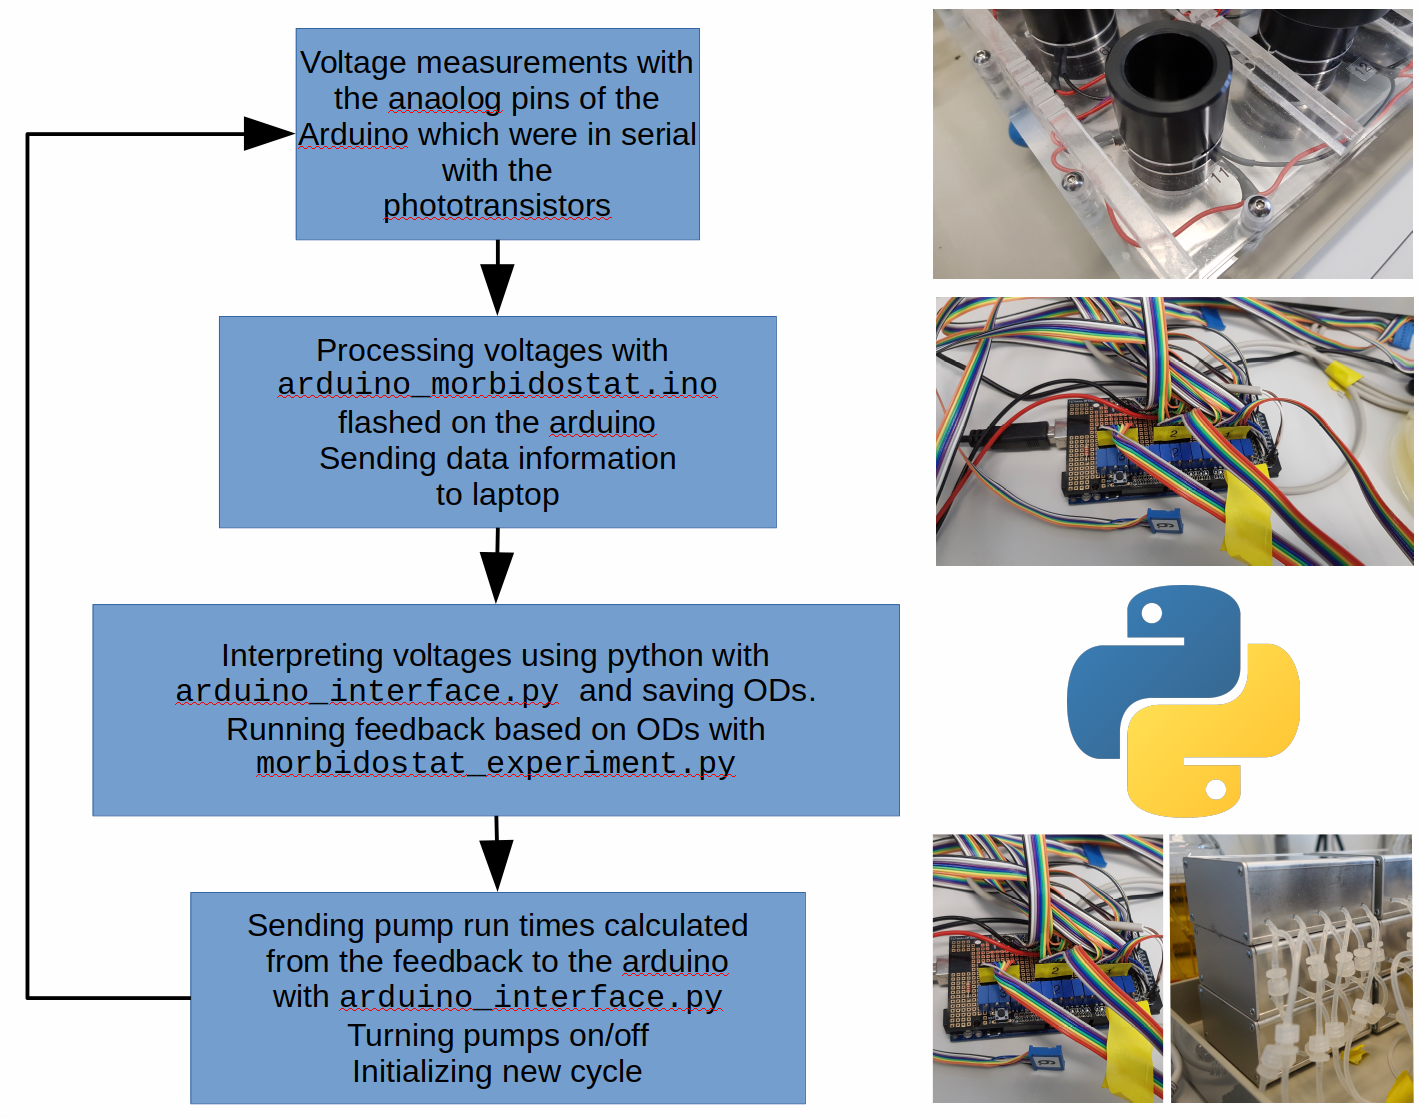
\includegraphics[scale=0.25]{flowchart.png}
	\caption{Overview of one cycle from the continuous mode of the morbidostat.}
	\label{figure:flowchart}	
\end{figure}

\subsubsection{Feedback of the continuous mode} 
The feedback determined how strongly the cultures were inhibited with antibiotics. This feedback was based on the relative difference between the averaged ODs of the current cycle and the averaged ODs of a past cycle. We called the average ODs of a cycle final\_OD and the relative difference between two final\_ODs \textDelta OD. 
\begin{center}
	$\Delta OD = (final\_OD_{x_{cycles\_back}} - final\_OD_{current\_cycle})/x$ \quad (3.1) 
\end{center}
As shown in Figure \ref{figure:feedback} the feedback did several comparisons before calculating an appropriate dose of antibiotics. As a first step it checked if \textDelta OD was positive or negative. A negative \textDelta OD implied that the bacteria were dying. In order to prevent complete sterilization, media was injected in this case, effectively diluting the antibiotic concentration in the vial. \\
When \textDelta OD was positive the bacteria were growing. Antibiotics were only injected if the bacteria reached a certain OD called drug\_dilution\_threshold. Therefore, the next comparison as visible in Figure \ref{figure:feedback}, was whether or not the final\_OD was bigger or smaller than this threshold. If the final\_OD was smaller no fluids were injected.
However when final\_OD was bigger than the threshold, calculation of the appropriate dose was initialized.
The calculation itself was split up into two equations.
\begin{center}
	$increase\_vial\_conc = vial\_conc + mic\_fraction*mic$ \quad (I) \label{eq:plus}
\end{center}
\begin{center}	
	$increase\_vial\_conc = vial\_conc * c * \Delta OD/target\_OD$ \quad (II) \label{eq:mult}
\end{center}
Equation I, mainly important at the beginning of the morbidostat experiments, was used to approximate the MIC of the strains in the vials. This was done by simply adding a fraction of the MIC (mic\_fraction) to the current vial concentration (vial\_conc). After the MIC was reached this equation was ignored and from now on equation II determined the injected concentration. This equation multiplied the current drug concentration in the vials (vial\_ conc) by the \textDelta OD which resulted in how much the drug concentration in the vial was increased (increase\_ vial\_ conc).
The goal of the feedback was that a certain OD called target\_OD was approximated in every vial. In order to do so we divided the second equation by this target\_OD. Now if a small target\_OD was chosen the increased concentration was divided by a small value causing a higher injected concentration. If target\_OD was set to a high value the divided outcome was smaller. As a last step a constant (c) was introduced, which allowed to fine-tune the aggressiveness of the feedback.   

\begin{figure}
	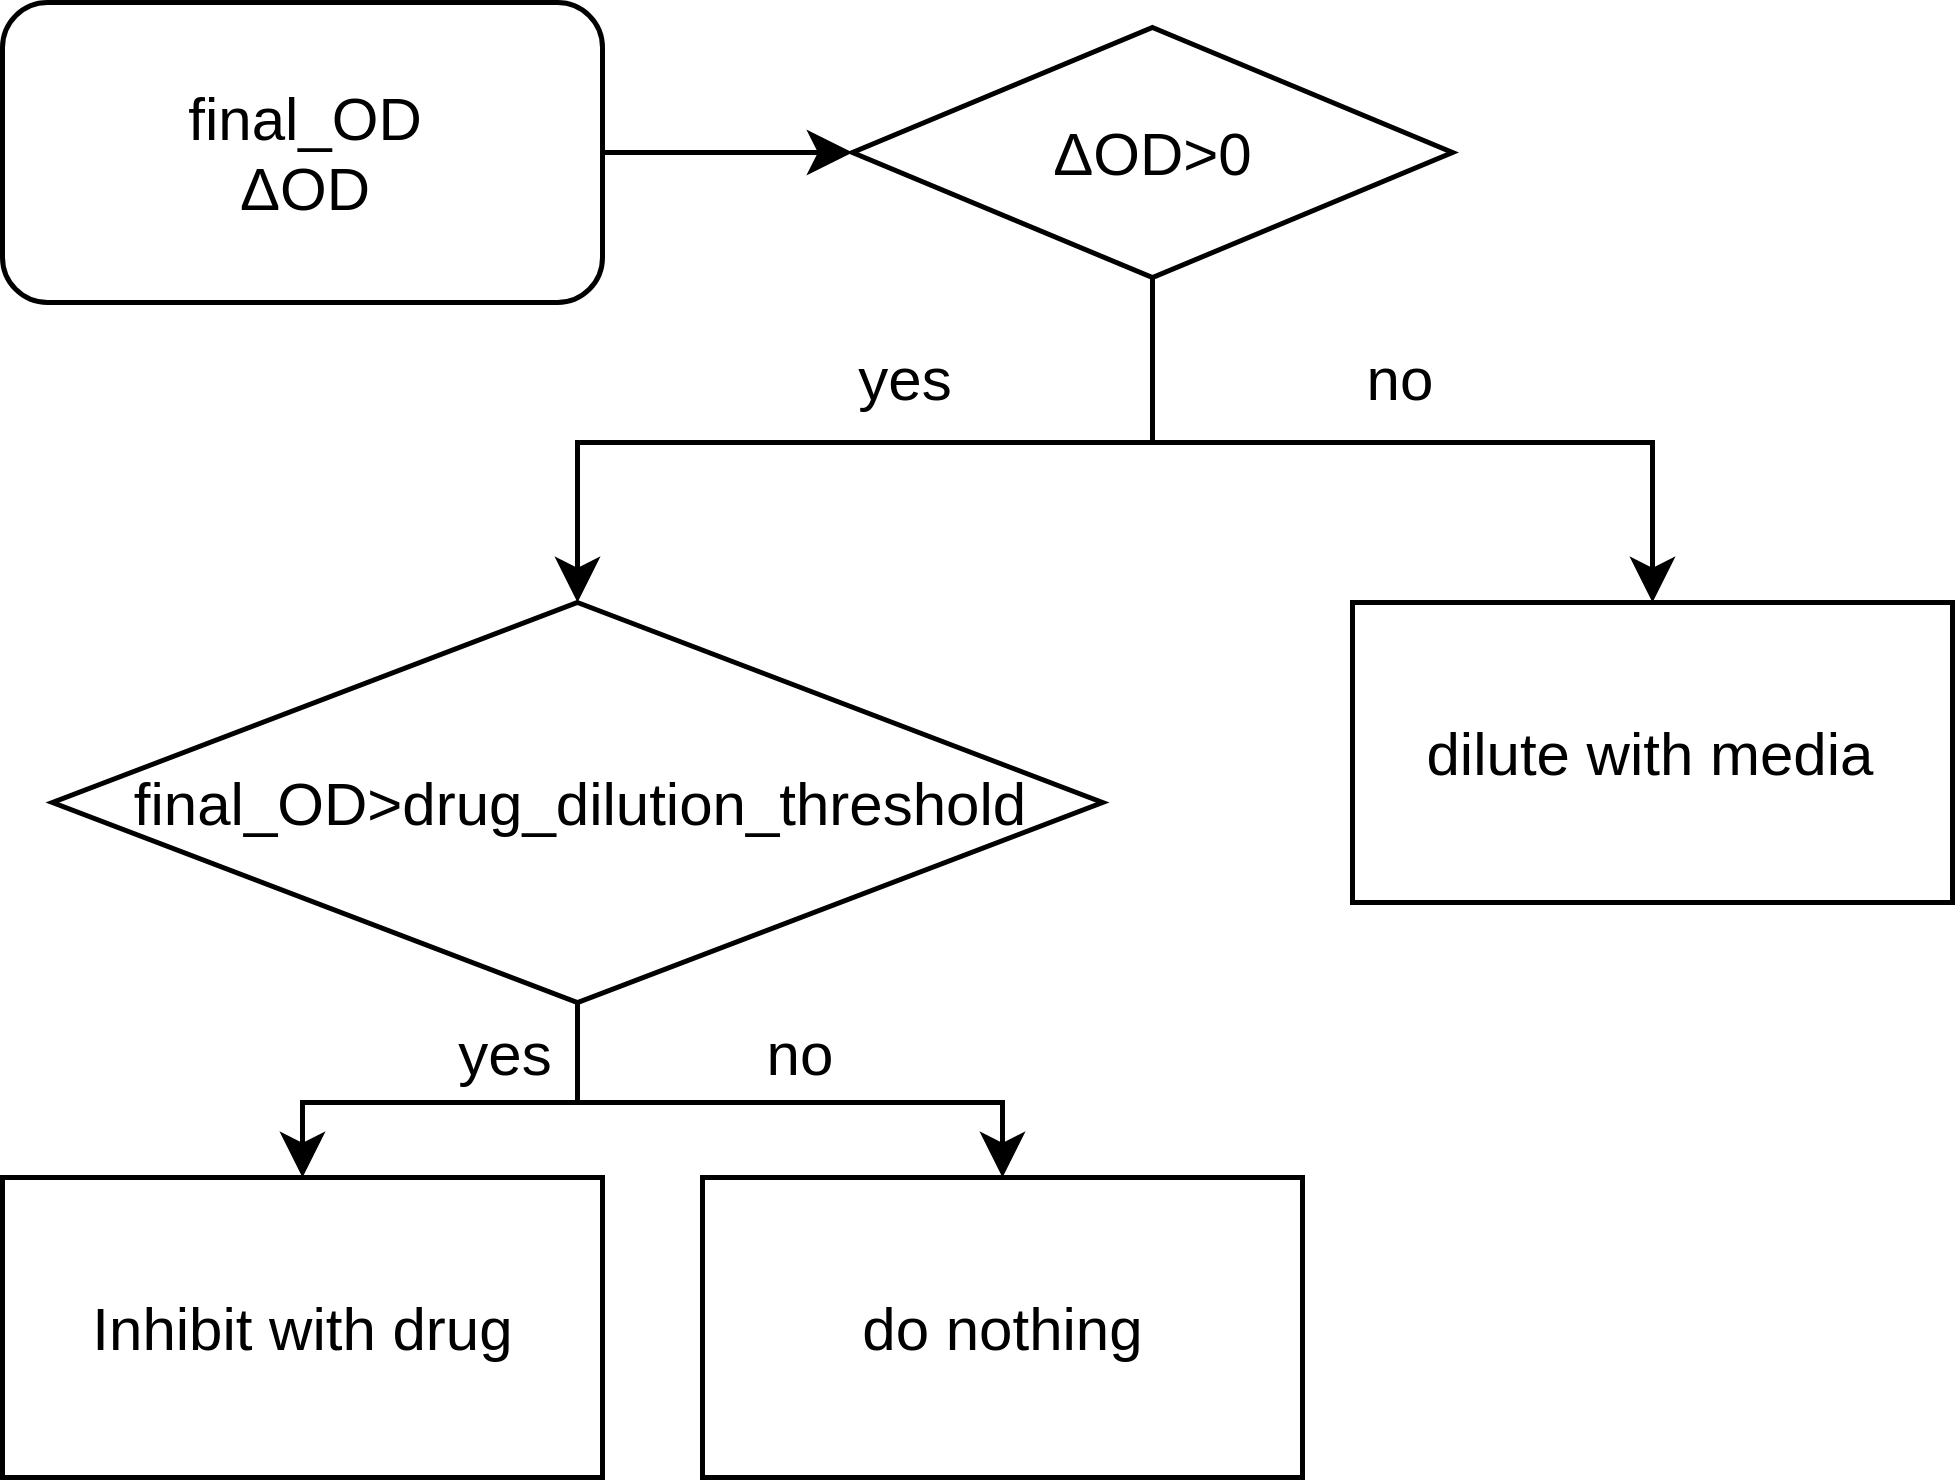
\includegraphics[scale=0.13]{feedback.png}
	\caption{Schematic overview of decisions involved in the feedback.}
	\label{figure:feedback}
\end{figure}

\subsection{Hardware calibration}
\subsubsection{OD and pump calibration}
The OD measuring units were calibrated by measuring several cultures with a known OD.
An overnight culture with K12 XL1 blue E. coli was inoculated in 5 ml 9/10 $H_2O$ and 1/10 LB media (also referred to as diluted media). The next day the overnight culture was diluted 1/200 in 50 ml diluted media. After a few hours of day culturing following OD standards were prepared with 18 ml diluted media in the vials for the morbidostat: 0.01 0.021 0.042 0.107 0.192 0.278\\
Then every vial with a certain OD was placed in every vial holder. With the function calibrate\_OD from the \href{https://github.com/nahanoo/ESBL\_project/}{morbidostat\_experiment.py}, a voltage measurement was done for every OD standard and every OD measuring unit. The result of this function was a linear equation which translated the voltages to ODs. \\
\begin{figure}[H]
	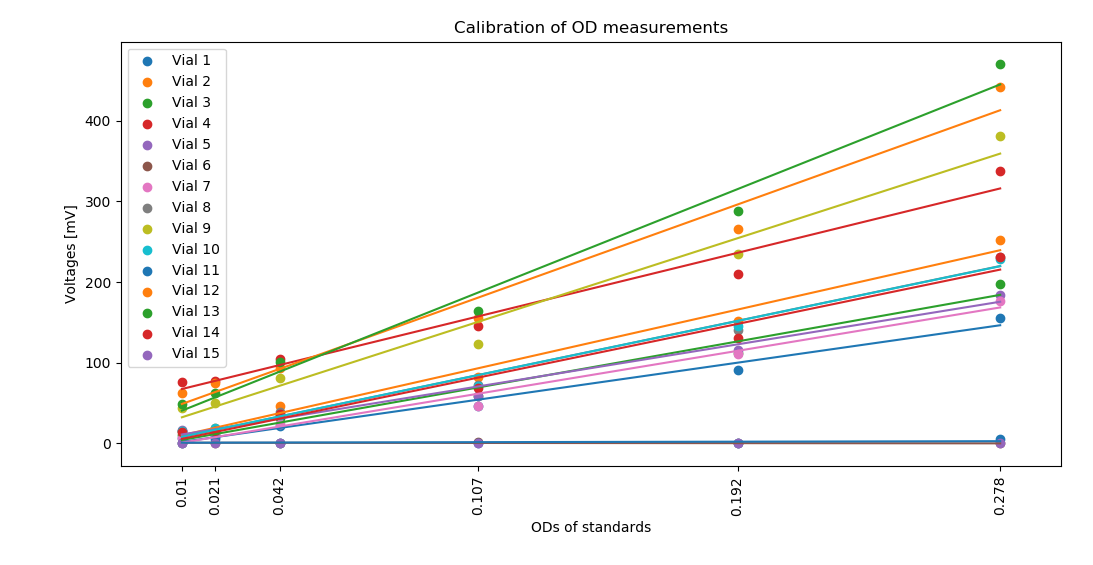
\includegraphics[width=1\textwidth]{od_calibration.png}
	\caption{Calibration of OD measuring units, with the OD standards on the x-axis and the measured voltages on the y-axis. The line represents the calculated linear equation. The units of vial 5 and 15 were not working.}
\end{figure}
To determine the flow rate of the pumps the function calibrate\_pumps from the\href{https://github.com/nahanoo/ESBL\_project/}{morbidostat\_experiment.py} was executed. The weight of every empty vial had to be entered and the function turned on every specified pump for 100 seconds. Afterwards the weight of the vials was entered again and the function calculated the flow rate for the specified pumps. 
\label{section:OD_calibration}

\section{Experimentally evolving resistance with the morbidostat}
For evolving resistance with the morbidostat Beatrice Claudi from Dirk Bumanns group  produced three ESBL \textit{E. coli} strains, by assembling ESBL producing plasmids with Gibson cloning which were transformed into \textit{E. coli K-12} MG1655 \cite{bioz.com_bioz_nodate}. Working with ESBL \textit{E. coli K-12} MG1655 increased the safety of the handling, because \textit{E. coli K-12} MG1655 does not colonize the human intestine.\\
We cultured the ESBL \textit{E. coli} strains with the plasmid produced with gibson cloning with the morbidostat in the continuous mode leading to increased resistance to cefepime within a few days. To confirm emerged resistance the MIC of the strains was compared before and after culturing with the morbidostat. Samples taken while culturing with the morbidostat were Illumina and ONT sequenced. The resulting sequencing data was analyzed using the bioinformatic pipeline described in Section \ref{section:pipeline}.

\subsection{Gibson cloning}
\begin{figure}
	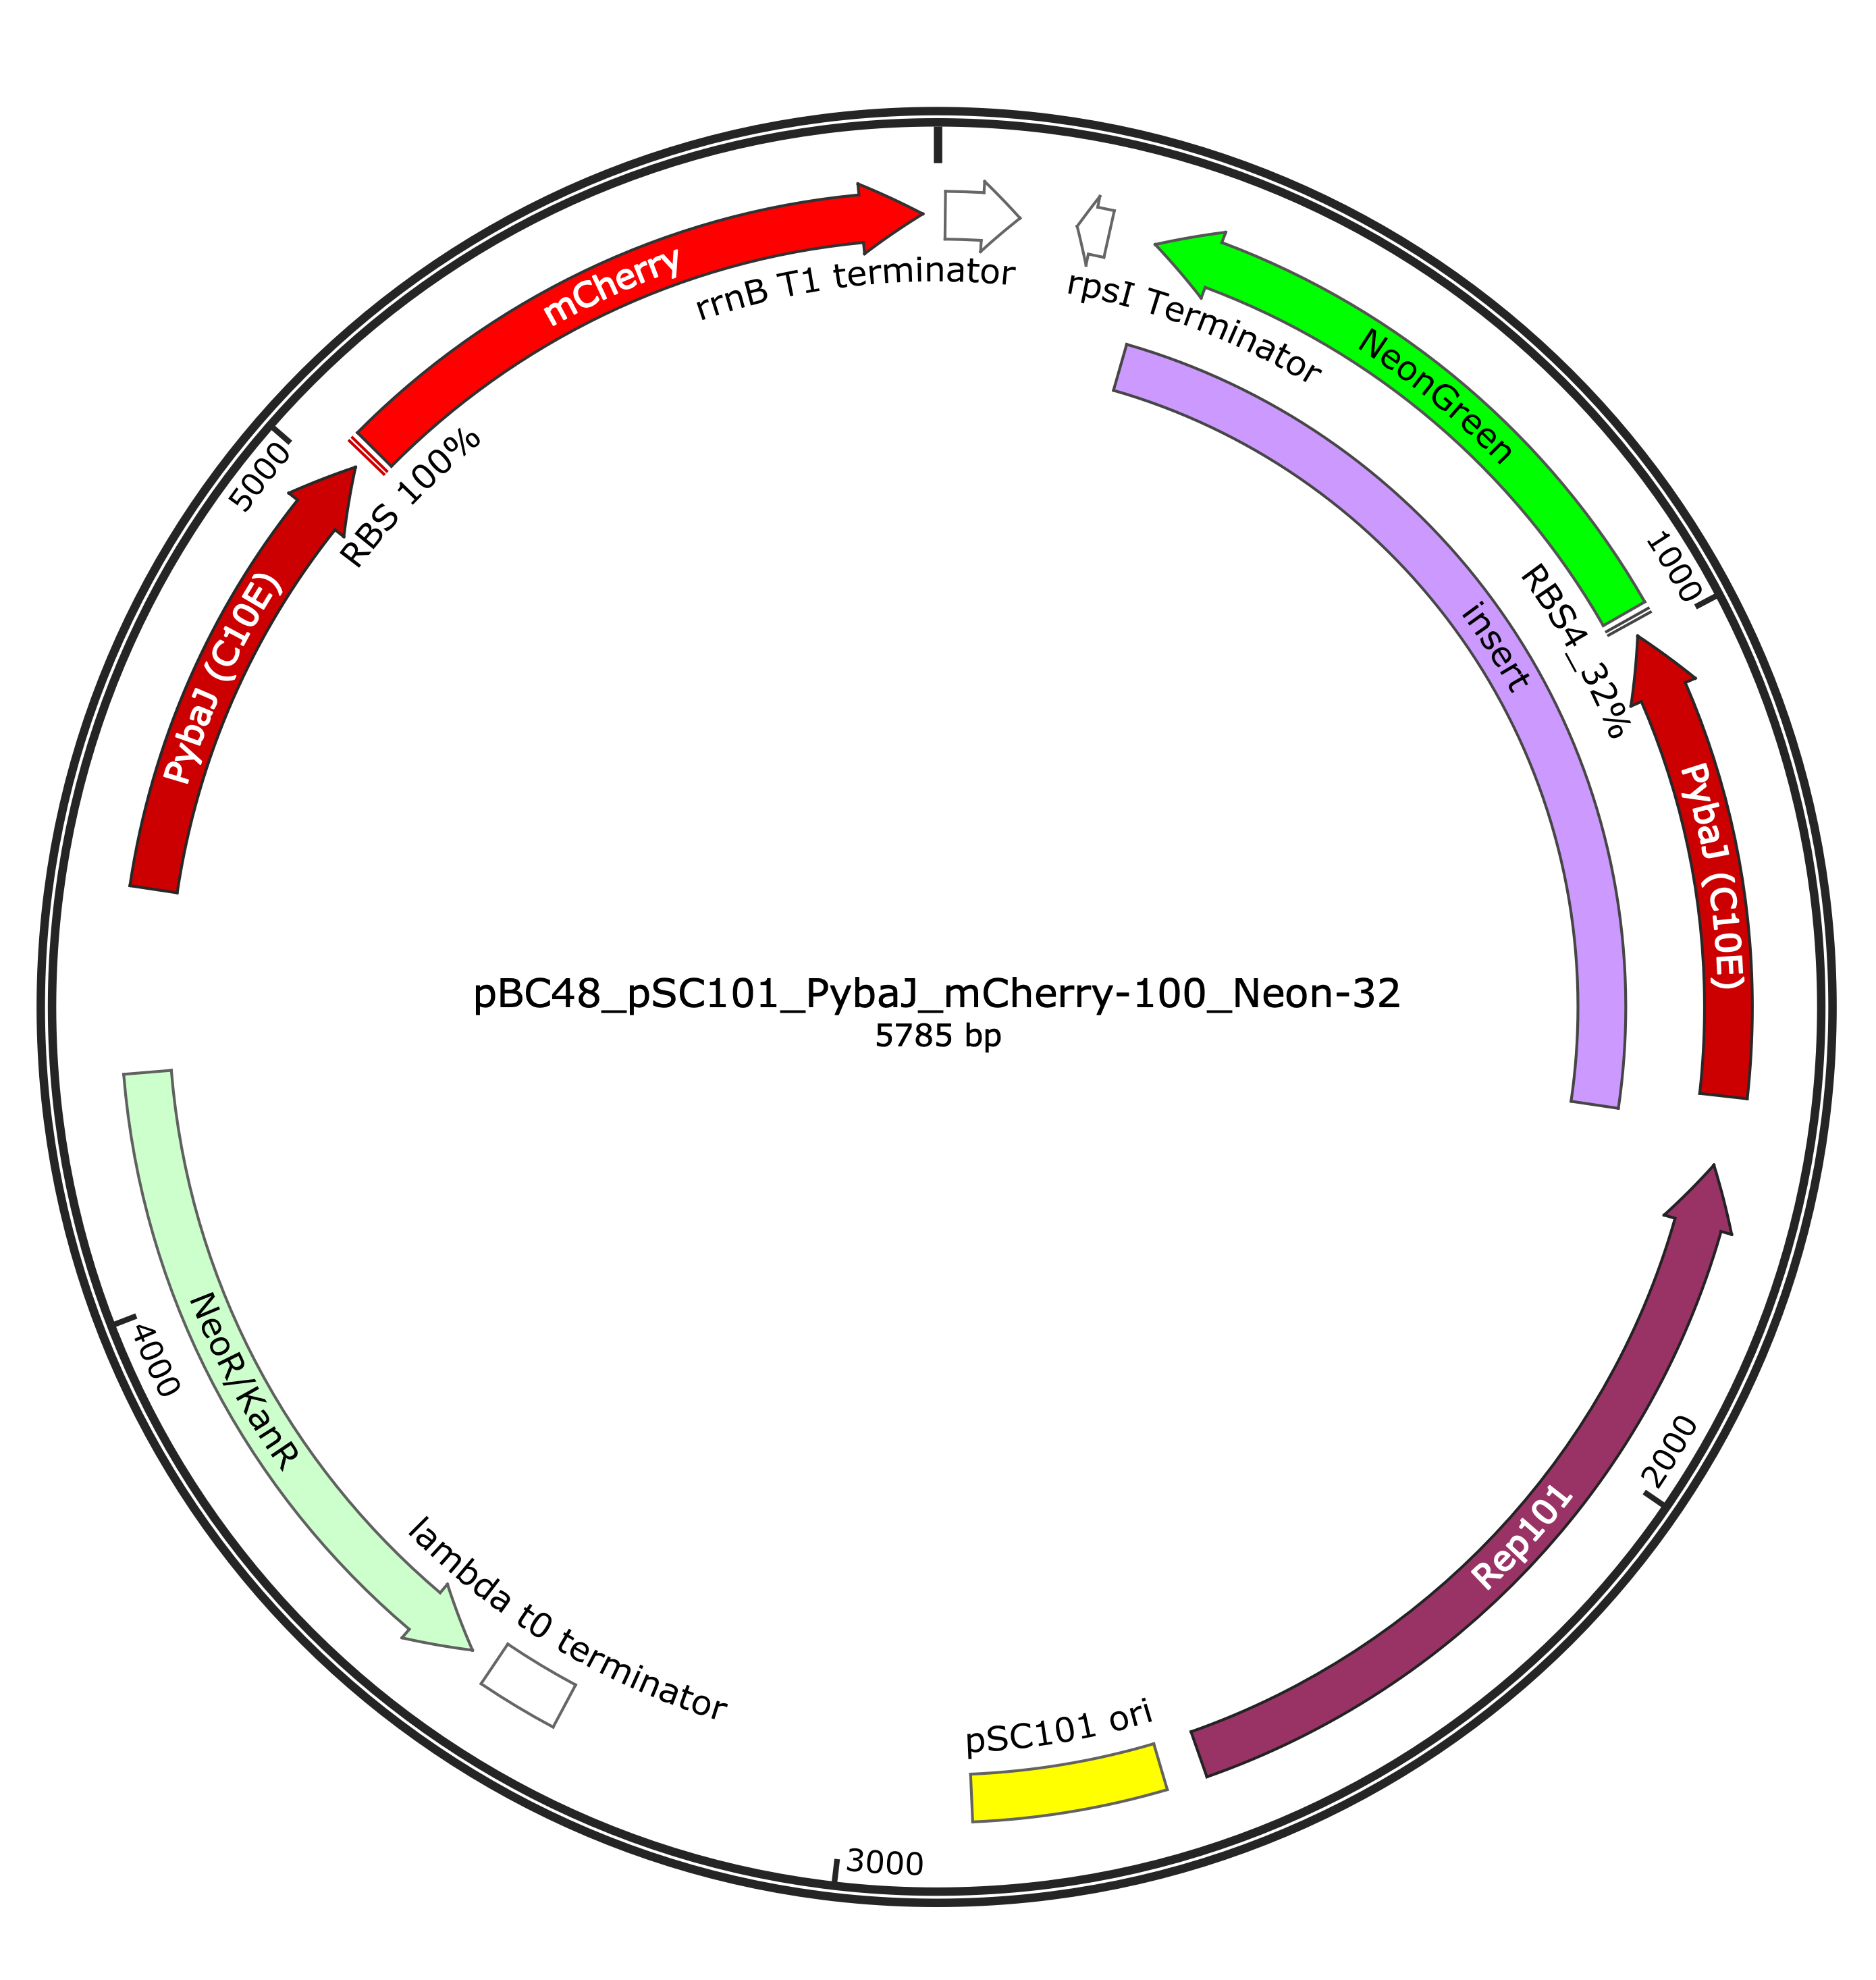
\includegraphics[width=0.45\textwidth]{pBC48_pSC101_PybaJ_mCherry-100_Neon-32_Map.png}
	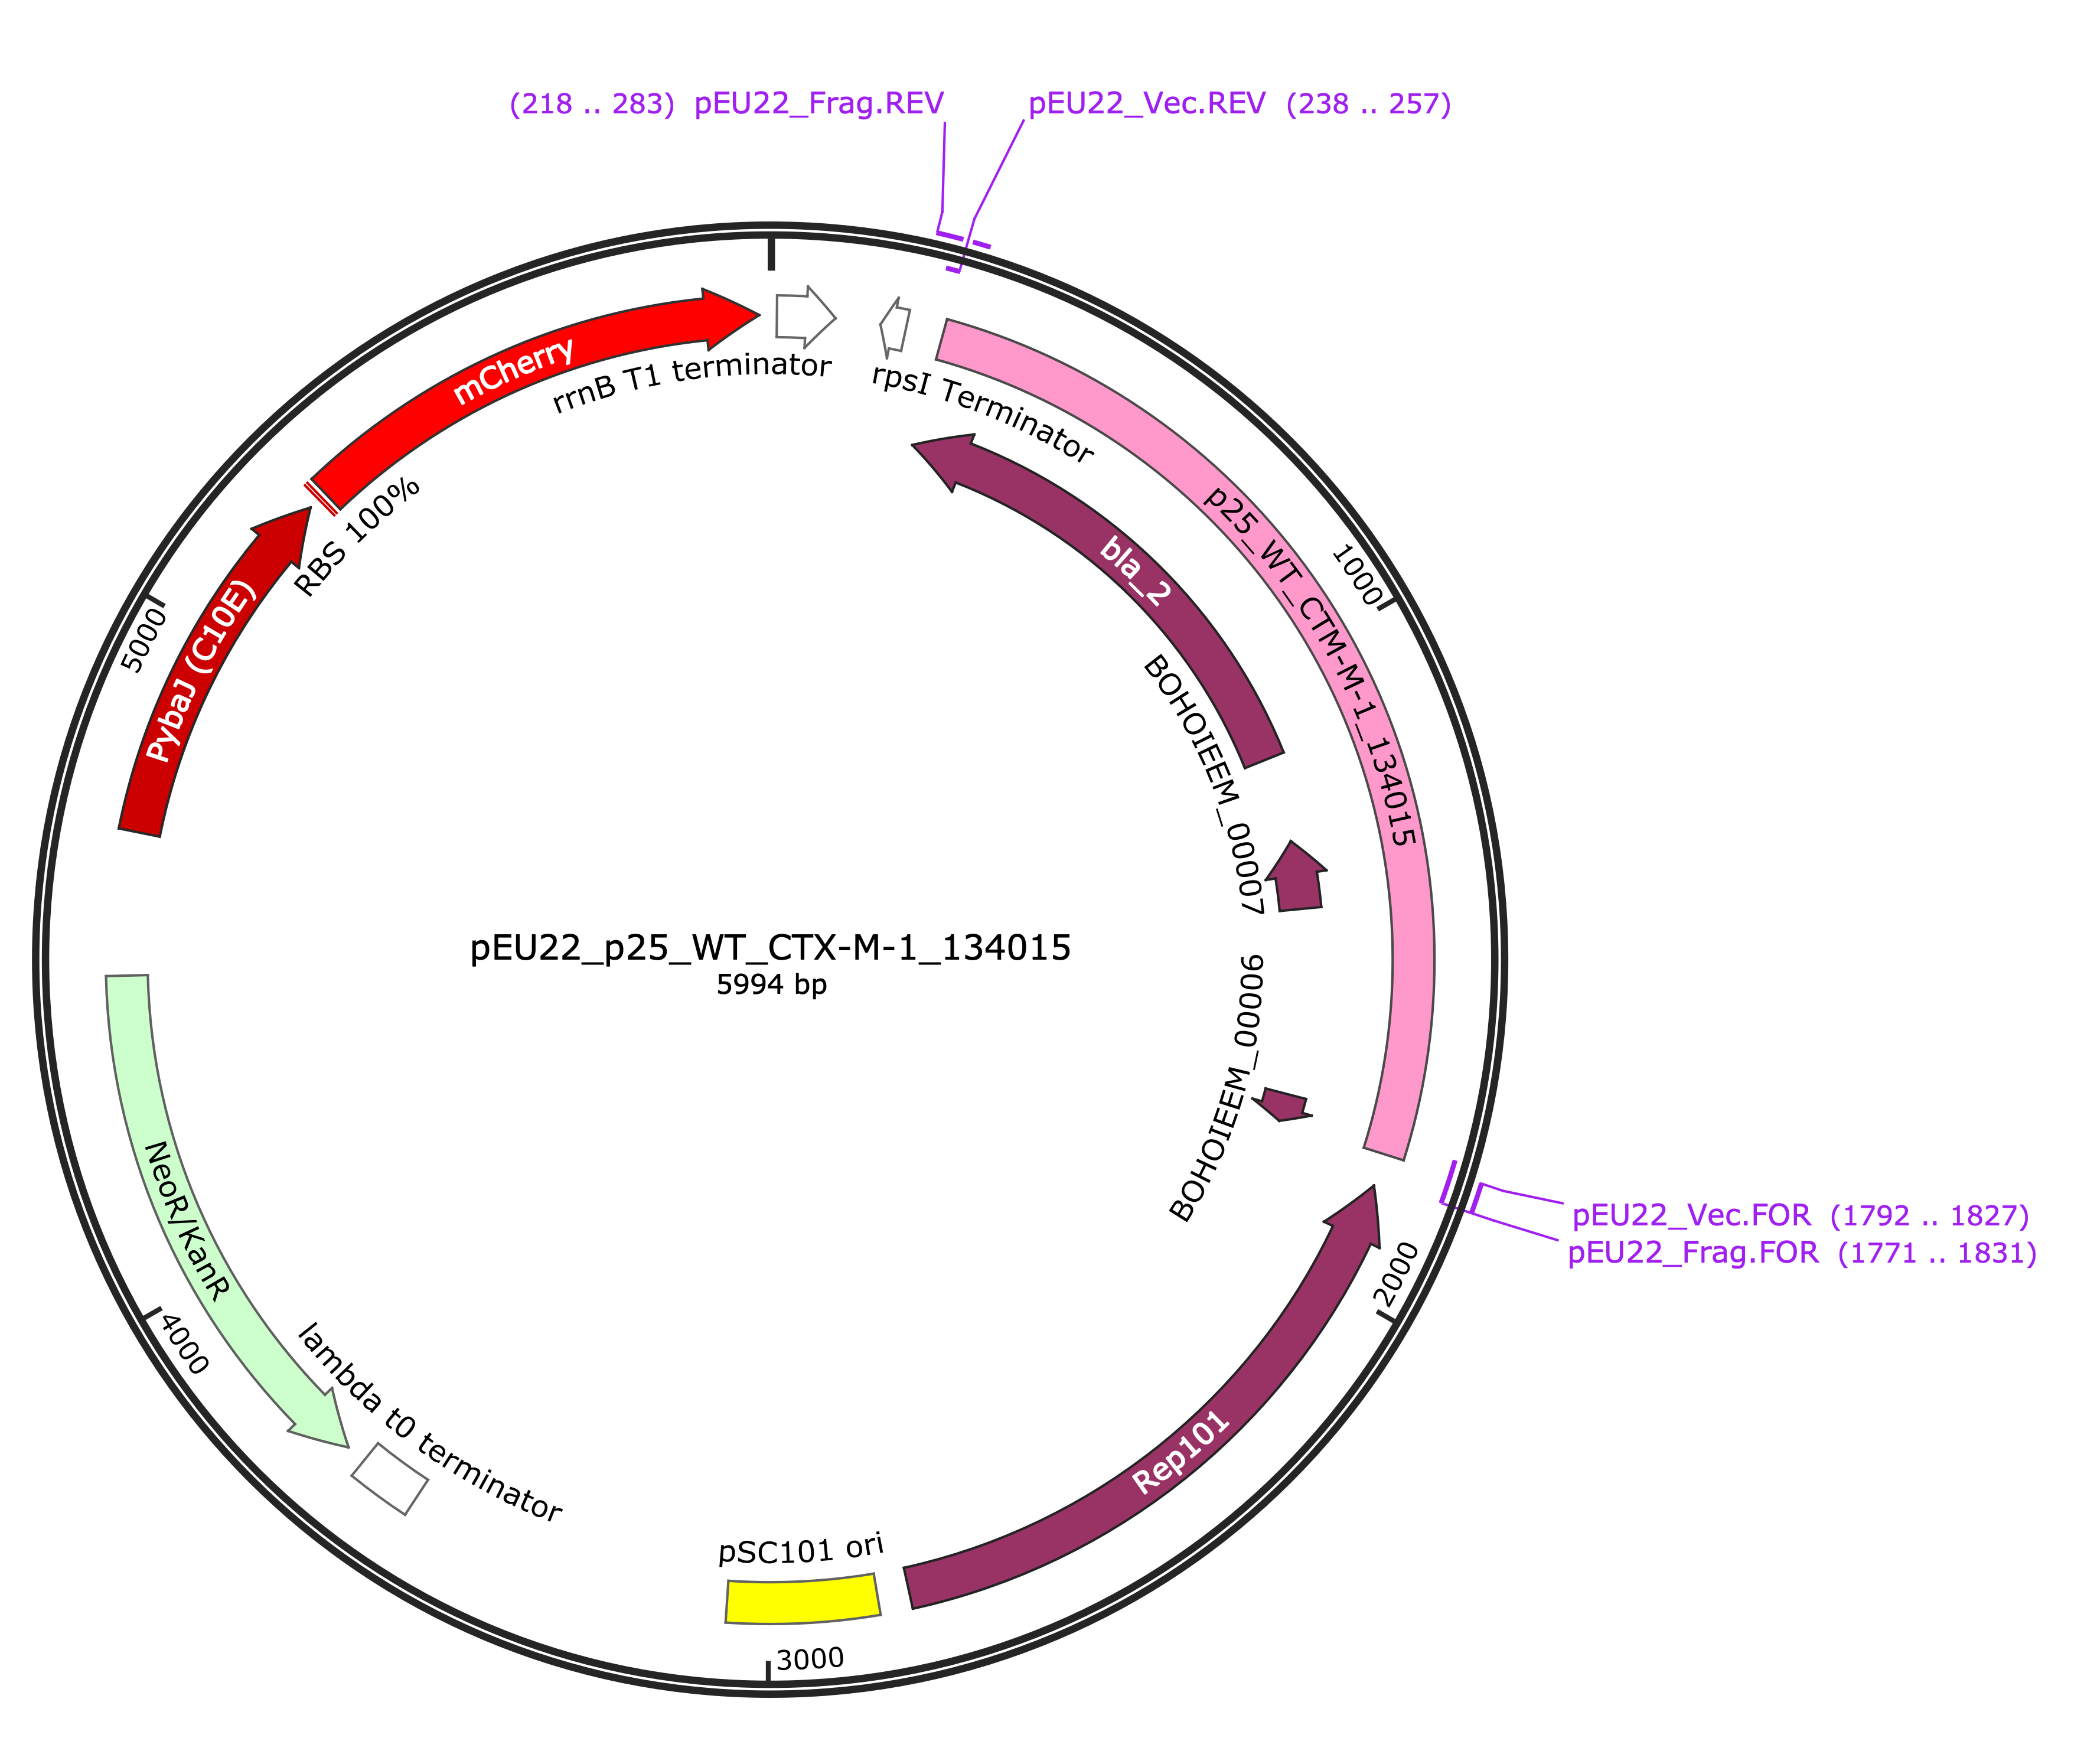
\includegraphics[width=0.55\textwidth]{pEU22_p25_WT_CTX-M-1_134015_Map.png}
	\caption{Left: Vector used for Gibson cloning. Right: Resulting pEU22 plasmid. The insert, consisting of an ESBL gene and its regulatory sequence amplified with template DNA from patient isolates, replaced NeonGreen which allowed selection for clones with the insert.}
	\label{figure:vec}
\end{figure}
We extracted three ESBL gene sequences and their upstream sequence up to the previous gene (regulatory sequence) from two isolates of the isolate collection from the University Hospital of Basel (see Section \ref{section:sample_collection}). An identifier was created for every extracted gene with its regulatory sequence. The extracted sequences are shown in the supplementary in Section \ref{section:sequences}. Primers for PCR amplification were designed, based on the extracted sequences.
\begin{table}[H]
	\begin{tabular}{|llll|} \hline
		ID    & Product                & Source             	& Fragment size in bp \\ \hline
		pEU22 & \textbeta-lactamase CTX-M-1 & Patient 25 isolate 1 &	1614 \\ \hline
		pEU23 & \textbeta-lactamase OXA-1   & Patient 25 isolate 1 & 1789\\ \hline
		pEU26 & \textbeta-lactamase OXA-1   & Patient 33 isolate 1 & 1789\\ \hline
	\end{tabular}
	\label{table:plasmid}
	\caption{Designed insert for gibson cloning. The ESBL genes were amplified including its regulatory sequence. }
\end{table}
\begin{table}[H]
	\begin{tabularx}{\textwidth}{|ccL|}
		\hline
		ID    & Direction & Primer sequence                                                                        \\ \hline
		pEU22 & Reverse   & cgaagcagaaccccaTCATCCGAGAGCTTGCATGCC TGCAttacaaaccgtcggtgacgattttag             \\ \hline
		pEU22 & Forward   & GGCTCTTGTATCTATCAGTGAAGCATCAAGACTAAC AAATgcccacagaatgatgtcacgc                  \\ \hline
		pEU23 & Reverse   & cgaagcagaaccccaTCATCCGAGAGCTTGCATGCC TGCAttataaatttagtgtgtttagaatggtgatcgcatttt \\ \hline
		pEU23 & Forward   & GGCTCTTGTATCTATCAGTGAAGCATCAAGACTAAC AAATgtgatcccctgggcgaaatg                   \\ \hline
		pEU26 & Reverse   & cgaagcagaaccccaTCATCCGAGAGCTTGCATGCC TGCAttataaatttagtgtgtttagaatggtgatcgcatttt \\ \hline
		pEU26 & Forward   & GGCTCTTGTATCTATCAGTGAAGCATCAAGACTAAC AAATgtgatcccctgggcgaaatg                   \\ \hline
		Vector & Forward   & GGCTCTTGTATCTATCAGTGAAGCATCAAGACTAAC AAATgtgatcccctgggcgaaatg                   \\ \hline
		Vector & Reverse   & GGCTCTTGTATCTATCAGTGAAGCATCAAGACTAAC AAATgtgatcccctgggcgaaatg                   \\ \hline
	\end{tabularx}
	\label{table:primer}
	\caption{Primers used for the PCR amplification of the ESBL genes with their regulatory sequence and for controlling the insertion into the vector.}
\end{table}
The fragments were amplified using the primer sequences shown in Table \ref{table:primer} and the KOD-Hot-start-DNA plymerase with template DNA from the according isolate.
The vector shown in Figure \ref{figure:vec} was amplified by PCR as well using the iProof fidelity polymerase, its sequence is shown in the supplementary (see Section \ref{section:sequences}). All PCR reactions were loaded on a 1\% agarose gel. Since only bands with the expected lengths were present, the bands were cut out and purified using the NucleoSPin Gel and PCR Clean-up Kit. The DNA was eluted in 30 \textmu L nuclease-free water. 
The following Gibson reaction was prepared in order to insert the fragments into the vector:
\begin{table}[H]
	\begin{tabular}{|llllll|}
		\hline
		\multirow{2}{*}{ID}    & \multirow{2}{*}{Fragment} & \multirow{2}{*}{Conc. [ng/\textmu L]} & \multicolumn{3}{l|}{Volume [\textmu L]}           \\
		&                           &                                       & DNA  & GIBSON MIX         & $H_2O$                  \\ \hline
		\multirow{2}{*}{pEU22} & Insert                    & 268                                   & 0.22 & \multirow{2}{*}{5} & \multirow{2}{*}{2.75} \\
		& Vector                    & 25.66                                 & 2.03 &                    &                       \\ \hline
		\multirow{2}{*}{pEU23} & Insert                    & 342.9                                 & 0.19 & \multirow{2}{*}{5} & \multirow{2}{*}{2.78} \\
		& Vector                    & 25.66                                 & 2.03 &                    &                       \\ \hline
		\multirow{2}{*}{pEU26} & Insert                     & 285.2                                 & 0.22 & \multirow{2}{*}{5} & \multirow{2}{*}{2.74} \\
		& Vector                    & 25.66                                 & 2.03 &                    &                       \\ \hline
	\end{tabular}
	\caption{Gibson reaction with the inserts, the vector and the GIBSON mix.}
\end{table}
The reactions were incubated for 20 min at 50 \degree C. From the reactions 2 \textmu L was added to 100 \textmu L electrocompetent cells of the strain \textit{E. coli K-12 MG1655}. The mixture was electroporated with a Bio-Rad electroporator, pelleted and resuspended in 1 mL super optimal broth. The cells were shaken for 2 hours at 180 rpm and 37 \degree C. The electroporated strains were plated on LB plates containing kanamycin  and grown over night. Because our vector includes a kanamycin resistance gene, all colonies which grew on the plates had the plasmid.  Additionally, the vector had two genes coding for fluorescence proteins, mCherry (red) and NeonGreen (green). As seen in Figure \ref{figure:vec} the insert replaced the gene coding for NeonGreen. Therefore the Gibson reaction was only successful for clones which were not green. Only red clones were picked and grown over night in LB containing kanamycin. Based on those cultures the clones were checked with a PCR. As a forward primer 'TCTCAATGGTTCGTTCTCATGG' was used, as a reverse primer 'GGAACAGTACGAACGCGCCGA' was used. The PCR control showed positive results and the strains were stocked in LB containing 20\% glycerol.
The ID created for the plasmids was adopted for the strains. 

\subsection{Culturing ESBL \textit{E. coli} strains with the morbidostat}
Before culturing with the morbidostat, we determined the MIC of the ESBL \textit{E. coli} strains and sterilized the device.

\subsubsection{MIC determination}
We inoculated 5 ml of MHB media with the ESBL \textit{E. coli} strains and cultured the suspension over night at 37 \degree C. The next day a 1/100 dilution in 20 ml MHB was prepared for every suspension and cultured for a few hours at 37 \degree C. The growth of the day cultures was constantly monitored by measuring the OD. When the OD of the day culture was 0.08, a 1/100 dilution of every day culture was prepared. \\
We added 100 \textmu L of MHB to every well of a 96 well plate. Except for the last column of the plate, we added 100 \textmu L of the diluted day culture to every well. 100 \textmu L of a cefepime solution with a concentration of 2.048 mg/mL was added to the first column of the plate. Starting from the first column a 1:1 dilution series was prepared with the the first seven columns. We incubated the plates for 16 hours at 37 \degree \space on a shaker. To get an idea how many cells were used for the MIC determination $10^{-3}$ and $10^{-5}$ dilutions of the 1/100 diluted cell cultures were plated on LB plates.\\
After 16 hours the OD of every well was measured using a plate reader. The smallest concentration which inhibited the growth was determined as the MIC. 
\label{section:mic_determination}

\subsubsection{Sterilization of the morbidostat}
We sterilized the morbidostat using two different disinfectants in order to prevent biofilm formation and contamination of our vials.
Bottles, vials, tubing and luer connections were autoclaved. Sterile vials were connected to the tubes and the computer controllable pumps were connected to 1 L of 3 \% citric acid stored in a sterile bottle with sterile tubing. All the tubing going to the vials was flushed with the disinfectant over one hour. The waste pump was turned on leading to disinfection of the tubes connected to the sterile waste bottle. After that the tubing was flushed with 1 L of sterile water. We repeated this procedure but this time using 3 \% of bleach as disinfectant.
\label{section:sterilization}

\subsubsection{Culturing with the morbidostat}
We ran two morbidostat experiments with the ID 01 and 02 with the ESBL \textit{E. coli} strains and \textit{E.coli K-12} MG1655 as a control. For every experiment we prepared over night cultures of the ESBL \textit{E. coli} strains in 3 ml diluted media with 3 \textmu L kanamycin. \textit{E. coli K-12} MG1655 was cultured over night in 3 mL diluted media. The over night cultures were diluted 200 fold the next day and cultured for a few hours. From those cultures, 200 \textmu L were transferred into sterile vials containing 18 mL diluted media. We prepared two different antibiotic concentrations which were connected to the pumps. We prepared a concentration of 9 \textmu g/ml cefepime in 1 L diluted media as a low-concentrated antibiotic solution. For the high-concentrated solution we prepared a cefepime concentration of 21 \textmu g/mL in 1 L diluted media. The morbidostat experiments were initialized with a target\_OD of 0.12, and a dilution factor of 0.91. Every ESBL \textit{E. coli} strain was cultured at least three times with the continuous mode. Additionally we cultured every ESBL \textit{E. coli} strain with the fixed\_OD mode. The temperature inside the hypoxi-station was set to 37 \degree C. The $O_2$ level was fixed to 10 \% and $CO_2$ fixed to 5 \%. \\
As resistance evolved the antibiotic concentrations of the bottles were changed. We checked which concentration was necessary to strongly inhibit the cultures. New cefepime concentrations which were 3 fold and 7 fold higher than the newly determined inhibiting concentration were prepared and connected. We changed the antibiotic concentrations of the bottles approximately every third day. If the suspension in the vials was extremely milk caused by dead cells we transferred 200 \textmu L of the suspension to a new sterile vial containing 18 ml diluted media.  \\
During both experiments we took daily samples by opening the vial in the hypoxi-station and transferring 1 mL to an eppendorf tube. The collected samples were centrifuged at 13'000 rpm for 10 minutes and resuspended in 200 \textmu L LB containing 20 \% glycerol. Those suspensions were frozen at -80 \degree C.\\

\subsection{Analysis of the morbidostat samples}
\subsubsection{Illumina and Nanopore sequencing}
We handed the stocks of the cloned ESBL \textit{E. coli} strains and K-12 MG1655 to our collaborators of the University Hospital of Basel where they were sequenced on a MiSeq-Illumina system (see Section \ref{section:illumina}).
Furthermore, we handed them the stocks for Illumina sequencing of the last sample day of every vial form the 01 experiment. 
From the 02 experiment we selected the stocks from vial 3,4,5,7 and 8 from the third sample day and the stocks from every vial of the last sample day for Illumina sequencing. Every stock that we handed over for Illumina sequencing was stroked out. 
We sequenced the ESBL \textit{E. coli} stocks and K-12 MG1655 with ONT. For DNA extraction we inoculated 3 mL LB containing 1 \% kanamycin with the ESBL \textit{E. coli} stocks. K-12 MG1655 was inoculated in 3 mL LB. The suspensions were cultured over night. The DNA of the resulting over night cultures was extracted following the protocol of the DNeasy Blood \& Tissue Kit (50). The extracted DNA was sequenced with a MinION as described in Section \ref{section:nanopore_sequenicng}. 

\subsubsection{Contamination analysis}
On the plates where we stroked out every stock that we handed over for Illumina sequencing we saw colonies which had a different shape than \textit{E. coli}. Therefore, we had the suspicion that some stocks were contaminated. Because we had Illumina sequencing data for every stock we could identify the contamination by blasting a few reads \cite{madden_blast_2003}. This revealed that the contamination was \textit{Bacillus cereus}. To identify which samples were contaminated, all the Illumina short-reads from every stock  were mapped to a \textit{Bacillus cereus} reference genome obtained from NCBI \cite{noauthor_bacillus_nodate} and the ESBL \textit{E. coli} reference genome produced with hybrid-assembling.

\subsubsection{Identifying mutations in morbidostat samples}
The sample series from the morbidostat experiments were analyzed following the bioinformatic pipeline described in Section \ref{section:pipeline}. 